% --------------------------------------------------------------------

\chapter[Transients]{Eruptive and Explosive Transients}
\def\chpname{transients}\label{chp:\chpname}

Chapter editors:
\credit{ebellm},
\credit{fedhere}

Contributing Authors:

\credit{arcavi},
\credit{chomiuk},
\credit{Doctor},
\credit{Fong},
\credit{Haiman},
\credit{Kalogera},
\credit{AshishMahabal},
\credit{raffaellamargutti},
\credit{tmatheson},
\credit{StephenRidgway},
\credit{ohadshemmer},
\credit{nathansmith},
\credit{paulaszkody},
\credit{Trimble},
\credit{svalenti},
\credit{Zauderer}

% \section*{Summary}
% \addcontentsline{toc}{section}{~~~~~~~~~Summary}
%
% Executive summary goes here, highlighting the primary conclusions from
% the chapter's science cases. This should be abstract length, no more:
% say, 200 words.

% --------------------------------------------------------------------

\section{Introduction}


Explosive and eruptive transients are physically and
phenomenologically diverse.   What these events share
are rare, large-amplitude deviations from a quiescent state.  These
outbursts are typically unpredictable and of limited duration, and so their
discovery and characterization are sensitive to the detailed observing
strategy.  Often, followup observations with other facilities can provide
significant additional scientific value, but this creates a challenge to
identify candidate events while they are still visible.

Transients such as novae, supernovae (SNe), and long gamma-ray bursts (GRBs)
probe the final stages of stellar evolution. Tidal Disruption Events
(TDEs), short GRBs, and
Cataclysmic Variables (CVs) give us the opportunity to study
compact and binary objects. Massive star eruptions allow us to understand
mass loss mechanisms and chemical enrichment.
The brightest transients (GRBs, TDEs,
SNe) are light beams that can be seen over cosmic distances, and some
transients---most notably Type Ia SNe---are cosmological tracers.
In this chapter we focus on LSST's potential to advance the astrophysics of
eruptive and explosive transients; the use of SNe for cosmology is
discussed in \autoref{chp:cosmo}. Transients in the Milky Way Disk are
discussed in more detail in \autoref{chp:galaxy}.

Cadence choices will determine LSST's ability to discover, classify, and
characterize these events. However, due to their different time scales,
different phenomena will benefit from different sampling
strategies---sometimes
significantly different, and at times orthogonal.  Competing objectives
described in this chapter are at the heart of LSST's observing strategy and
cadence design.

When evaluating a particular observation or series of observations in
light of how they perform for a specific science case, it may be
helpful to think of metrics as lying along a continuum between
discovery and characterization. Discovery requires a minimum amount of
information to recognize an event or object as a candidate of
interest.  It is particulary relevant for science cases that require
triggering followup resources in real time from the live event stream.

Characterization, on the other hand, implies
that basic properties of the event may be determined from the
LSST observations, including but not limited to the classification of
the event.
It is particular relevant for science cases requiring analysis of large
samples of completed lightcurves.

Characterization and classification of transient events
benefits from substantial temporal sampling over the finite duration of the
event along with color information (perhaps contemporaneous).
Transient events slower than $\sim$ weeks may be adequately sampled by
a uniform LSST cadence.  Obtaining adequate sampling for faster-evolving
events may require special scheduling
strategies.  For some event types, LSST can only be expected to
provide a discovery service, and followup will necessarily be
performed elsewhere---so long as the cadence is sufficient to identify the
event type.
For some events, such as detecting electromagnetic counterparts to
gravitational wave events (GWs),
serendipitous discoveries are unlikely, but
enabling a ToO program would provide the opportunity for LSST to
contribute significantly to this science.

%The interpretation of a given metric along this continuum has
%implications for the subsequent action and analysis required,
%particularly as regards possible follow-up observations with other
%facilities.

We consider a non-exhaustive set of ``astronomical transients'' in the
paragraphs that follow. For a few of these transients, we quantify the
ability of LSST cadences to produce data useful for various science
goals. These case studies include SNe, GRBs, and GWs. For other
transient families (Novae, LBVs, TDEs) we provide more general
information in \autoref{sec:\chpname:future}, and we invite the
community to further develop the ideas proposed here, as well as
further other related goals, into quantified science cases.

\subsection{Targets and Measurements}
\label{sec:\chpname:targets}

%The class of transients includes a heterogeneous assortment of objects
%and phenomena.
\autoref{tab:transient_types} is a \emph{non-exhaustive} list of
phenomena to which we are referring as \emph{eruptive and explosive
  transients} in this document.

  \begin{table}
\begin{center}
  \begin{tabular}{| p{4.0cm} | p{4.0cm} | l | l | p{1.5cm}|}
    \hline

    Transient Type & Science drivers & Amplitude & Time Scale & Event Rate\\
\hline

Flare stars & Flare frequency, energy, stellar age, space weather & large &
	  min & very common\\

X-ray Novae & Interacting binaries, stellar evolution, SN progenitors,
nuclear physics & large & weeks & rare\\

Cataclysmic variables (\ref{sec:\chpname:CVtransients})& Interacting binaries, stellar evolution, compact
objects & large & min - days & common\\

LBV variability (\ref{sec:\chpname:LBVs})& Late stages stellar evolution, Mass loss, SN progenitors
& large & weeks-years & rare \\

Massive star eruptions (\ref{sec:\chpname:LBVs})& Late stages stellar evolution, Mass loss, SN progenitors & extreme & weeks-years & rare\\

Supernovae (\ref{sec:\chpname:SNtransients})& stellar evolution, feedback, chemical enrichment, cosmology & extreme & days - months & very common\\

GRBs (\ref{sec:\chpname:grbs})& jet physics, SN connection, stellar evolution & extreme & min - days
	  & rare (optical discovery) \\

TDEs (\ref{sec:\chpname:tdes})& Massive BH demographics, accretion physics & large & weeks-months & very rare\\


LIGO detections (GW, \ref{sec:\chpname:gw}) & EM characterization & unknown
	  & unknown & very rare\\

\emph{Unknown} & Discovery & unknown & unknown & rare\\

 \hline \end{tabular}
\end{center}
\caption{Overiew of major types of optical transients.  Common events have
hundreds or thousands of exemplars, while rare event classes have only a
	  few or tens.
\label{tab:transient_types}}
\end{table}

\begin{figure}[hbt]
\centerline{
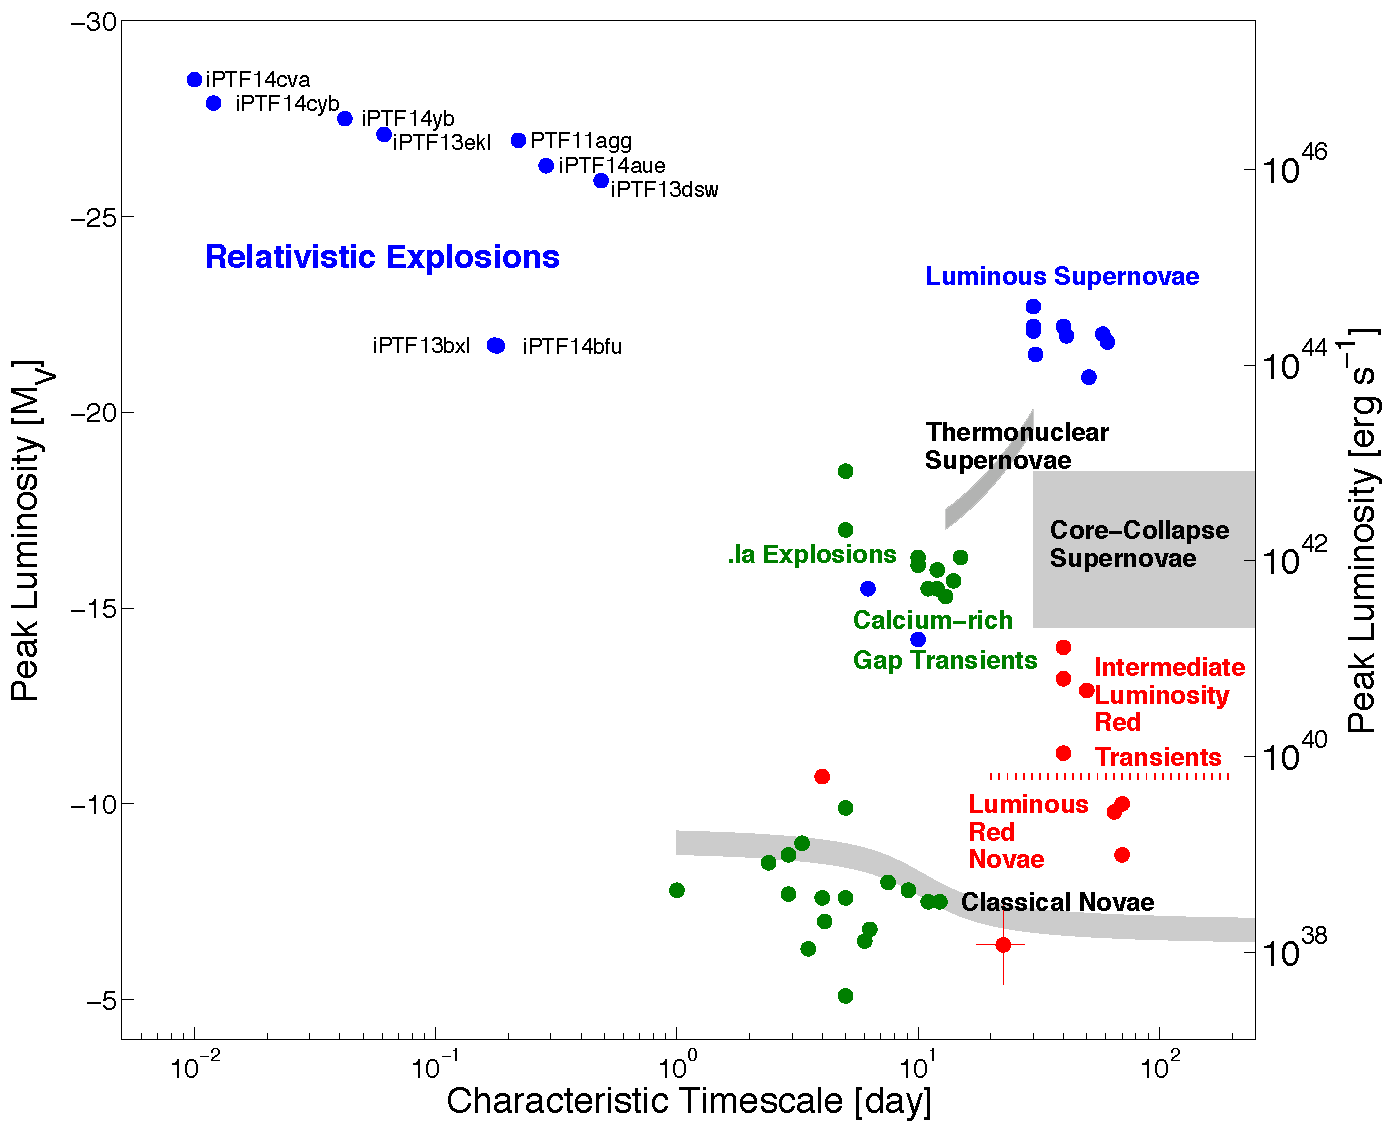
\includegraphics[width=0.6\textwidth]{figs/transients/taumv_2014.pdf}
}
\caption{
Peak luminosity-characteristic decay timescale plot for explosive
transients \citep[adapted from][]{2011PhDT........35K}.
}
\label{fig:transient_phase_space}
\end{figure}



%templates and stacks

%confusion

%


% --------------------------------------------------------------------


\subsection{Transient time scales}

Optical transients display a wide range of intrinsic timescales
(\autoref{fig:transient_phase_space}), and even some long-lived events
have short-duration features of interest.

For very short-lived phenomena (stellar flares, GRBs),
the main function of LSST will be to provide discoveries and/or simple
characterization.  Followup to discovery/identification, if required,
must take place elsewhere. This implies that the LSST observations
must be sufficient to recognize in real time that an event is fast-evolving
in order to to trigger followup. However, assessing the rise
slope is best done with a single filter,
because when observing with different
filters it is very difficult to separate lightcurve evolution from
color variations. Colors are informative when considering statistical
samples (\autoref{sec:\chpname:SNtransients}) as long as the epoch of peak
can be reliably determined.

SNe fall in an intermediate time range.  LSST will provide
multiple visits in multiple filters during the typical SN duration
(months).  This sampling may still be insufficient for many science
objectives, such as photometric classification of SN subtypes.
However, moderate changes to LSST
observing strategy may enhance the sampling for part of the sky part
of the time, greatly improving the usefulness of SN observations.
Metrics that assess the discovery rate of SN are included in
\autoref{chp:cosmo}.
Here we are interested in assessing the ability of
LSST to discriminate SN from other transients, SN subtypes from one
another, and to identify particularly interesting SNe: for example
those that show signature of shock break-out, companion interaction
in the early light curve, or would be candidates for \emph{flash
spectroscopy} follow-up \citep[e.g.,][]{2014Natur.509..471G}.
In addition, metrics that
quantify LSST's ability to constrain SN physics in a statistically
large sample of SN are needed.

TDEs have only recently started to be characterized in the optical
bands. The current sample of events show relatively long
time-scales (rise and decline of the light curve is over months). We
would like to assess through metrics how well TDEs can be
distinguished from supernovae based on their light curve shape and
color (in real-time so that followup observations can be triggered)
and how well the LSST light curves themselves can be used to model the
TDE emission and deduce the black hole properties.
%Ref. Science Book:
%10.6.1, \citet{Gezari2012, Chornock2014, Arcavi2014, Holoien2014,
%Holoien2015, Holoien2016}.

Large amplitude flares from AGN may mimic
explosive transients; they are discussed in \autoref{chp:agn}.

In addition we hope that LSST will provide a wealth of serendipitous
discoveries of yet-to-be-observed transients.  An ideal transient
discovery survey would include balanced coverage of all time scales. LSST
will cover longer time periods well, but will have to make some
choices of emphasis in coverage of shorter time-scales.

In the sections that follow we will use several case studies to assess
LSST's performance for a range of time-domain science:

\begin{itemize}
\item
  The ability of a given LSST cadence to discriminate truly young
  transients from those only first detected well after their explosion date (\autoref{sec:\chpname:transientsAge}).
  This ability is a crucial input to follow-up strategy design.
  We identify a region of lightcurve slope
  % the phase-space of rising speed and color
  that is characteristic of a
  variety of transients in their early phases and assess the ability of LSST's
  cadences to place transients within this phase-space.
  More sophisticated classification algorithms will likely be necessary, but
  are beyond the scope of this whitepaper.
\item
  The statistical constraints to a transient class that can be obtained
  over the course of the LSST survey, from the LSST survey data alone
  (assuming a successful classification). We discuss SN Ia early interaction
  signatures and IIb shock break-out (\autoref{sec:\chpname:SNtransients}).
\item
  The ability to identify in real-time a rapidly-evolving
  object of interest and
  trigger prompt follow-up observations. For this topic GRBs are used as
  a case study (\autoref{sec:\chpname:grbs}).
\item
  The value of triggered Target-of-Opportunity observations for
  following up very rare, fast-evolving events.   Here the kilonova
  counterparts expected from Advanced LIGO triggers are used as a
  case study (\autoref{sec:\chpname:gw}).
\item
  The insight that a cadence gives into single transient classes. We
  discuss CVs, massive star eruptions, and TDEs (\autoref{sec:\chpname:future}).

\end{itemize}


% --------------------------------------------------------------------

\subsection{Metrics}
\label{sec:\chpname:metrics}

Two metrics were developed and are used in this chapter specifically for transient phenomena:
\begin{itemize}
  \item{\metric{transientAsciiMetric}: accepts an ASCII file in input, so that realistic transient shapes can be used, with different shapes for different filters. The output can be the series of LSST observations (magnitude and error), or the fraction of transients detected (with user-specified constraints). This metric is used in \autoref{sec:\chpname:SNtransients}.}
  \item{\metric{GRBTransientMetric}: calculates the fraction of GRB-like transients detected (with user-specified constraints) using an $F(t) \propto t^{-\alpha}$
    lightcurve. This metric is used in \autoref{sec:\chpname:grbs}}.
\end{itemize}

Additionally, the standard MAF metrics
that quantify the gaps between consecutive visits to
a field within a night and over multiple nights
(\MAFmetric{IntraNightGapsMetric} and \MAFmetric{InterNightGapsMetric})
are of great value and are
heavily used throughout this chapter, in \autoref{sec:\chpname:transientsAge},
~\autoref{sec:\chpname:SNtransients}, and~\autoref{sec:\chpname:gw} for example.
These quantify the median times between consecutive visits to a field
within one night and over multiple nights, respectively.

Further metrics relevant to transient science are discused in \autoref{chp:galaxy},~\autoref{chp:cosmo}, and ~\autoref{chp:variables}.

Many science cases can be developed and tested with these metrics, and we
encourage users to do so. In addition, we are collecting a library of representative transient lightcurves in a separate GitHub repository\footnote{\url{https://github.com/LSSTTVS/LSST_TVS_RoadMap}} and we encourage readers to contribute their transient models or observations.


% --------------------------------------------------------------------

\subsection{OpSim Analysis}
\label{sec:\chpname:analysis}

The current set of simulated cadences
provide poor coverage in any one
filter for transient events longer than a visit pair ($\sim$30
minutes) and shorter than $\sim$ weeks (\autoref{fig:tgaps} and
\autoref{fig:tgaps_r}; \autoref{tab:visitgaps}).

As discussed in the subsequent sections, this
gap in the sampling hinders characterization of fast-evolving
transients.  A cadence with two visits separated by an hour or two rather
than 20 minutes would provide better discrimination.  A third visit in the
same night in a different filter would provide
color information valuable for realtime classification.
If a subset of those third
visits were in the same filter as the first two, it would improve the shape
characterization of the fastest-evolving transients.

\begin{table}
  \begin{tabular}{l|p{6cm}|c|c|c|c|p{5cm}}
    FoM & Brief description & {\rotatebox{90}{\opsimdbref{db:baseCadence}}}
          & {\rotatebox{90}{\opsimdbref{db:NEOswithVisitTriplets}}} &
          {\rotatebox{90}{\opsimdbref{db:NoVisitPairs}}} &
          {\rotatebox{90}{\opsimdbref{db:opstwoPS}}} & Notes \\
    \hline

    \thesection-1 & \footnotesize{\MAFmetric{IntraNightGapsMetric},
    any filter}      & 0.39 & 0.42 & 0.18 & 0.40 &
    \footnotesize{Median gap (hours) between consecutive observations of a field
	    in any pair
    of filters in a single night.} \\

    \thesection-2 & \footnotesize{\MAFmetric{IntraNightGapsMetric},
    $r$ band}      & 0.40 & 0.44 & 0.17 & 0.41 &
    \footnotesize{Median gap (hours) between consecutive $r$-band observations of a
	    field in a single night.} \\

    \thesection-3 & \footnotesize{\MAFmetric{InterNightGapsMetric},
    any filter}      & 3.0 & 3.9 & 2.0 & 3.0 &
	    \footnotesize{Median gap (days) between consecutive observations of a field
	    in any pair
    of filters over multiple nights.} \\

    \thesection-4 & \footnotesize{\MAFmetric{InterNightGapsMetric},
    $r$ band}      & 15.0 & 22.8 & 11.0 & 21.9 &
    \footnotesize{Median gap (days) between consecutive $r$-band observations
    of a field over multiple nights.} \\

\end{tabular}
\caption{
Inter- and intra-night revisit metrics in any filter and in $r$-band for
several simulated surveys.
}
\label{tab:visitgaps}
\end{table}

\begin{figure}[hbt]
\centerline{
	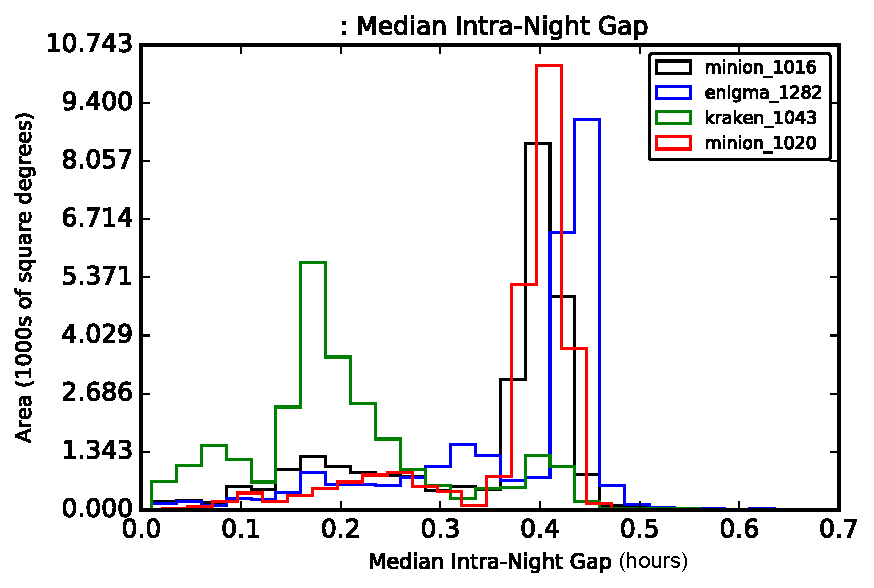
\includegraphics[width=0.45\textwidth]{figs/transients/MedianIntra-NightGap.pdf}
	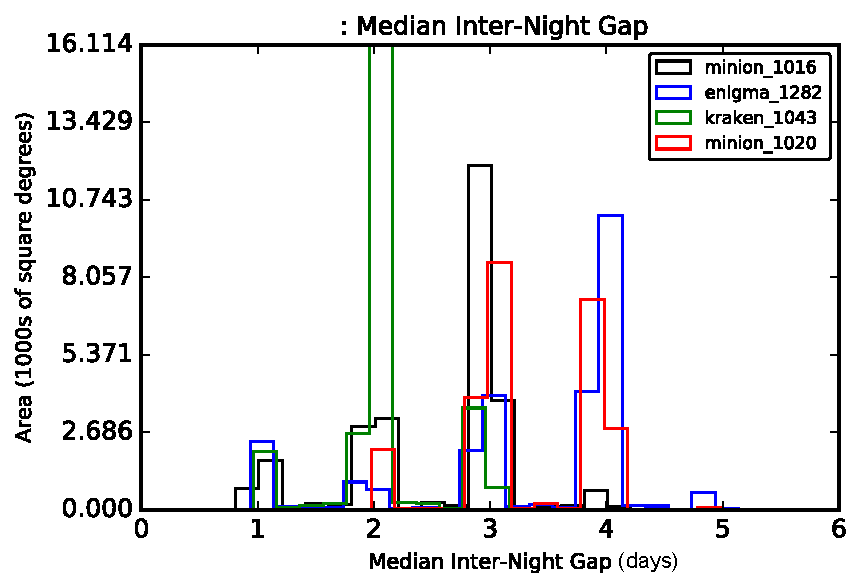
\includegraphics[width=0.45\textwidth]{figs/transients/MedianInter-NightGap.pdf}
}
\caption{ Histograms of median intra-night visit gaps (hours, left) and
	inter-night visit gaps (days, right)
for any band for several OpSim runs.  Current simulations provide little
	temporal coverage for transient timescales between 30 minutes and
	2--3 days.}
\label{fig:tgaps}
\end{figure}

\begin{figure}[hbt]
\centerline{
	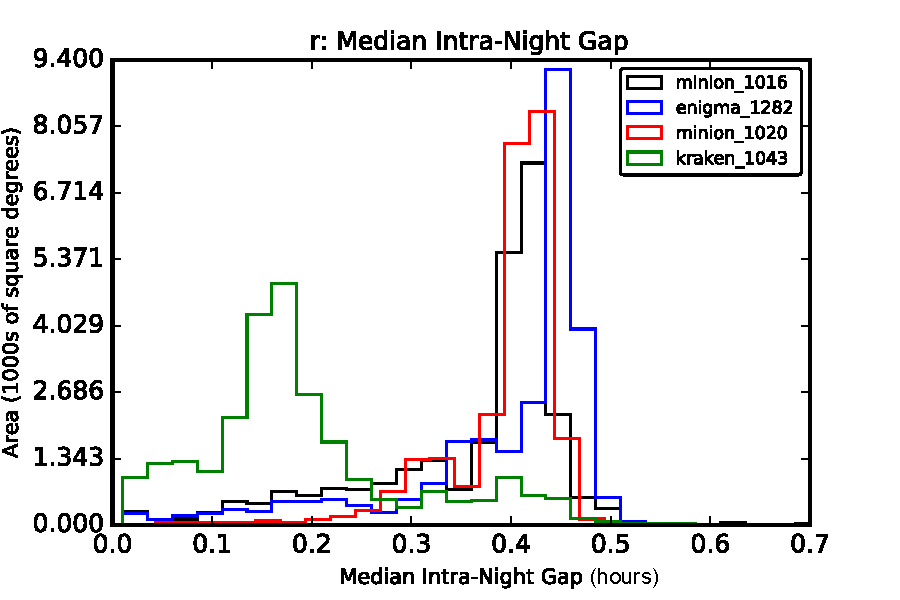
\includegraphics[width=0.45\textwidth]{figs/transients/MedianIntra-NightGap_r.pdf}
	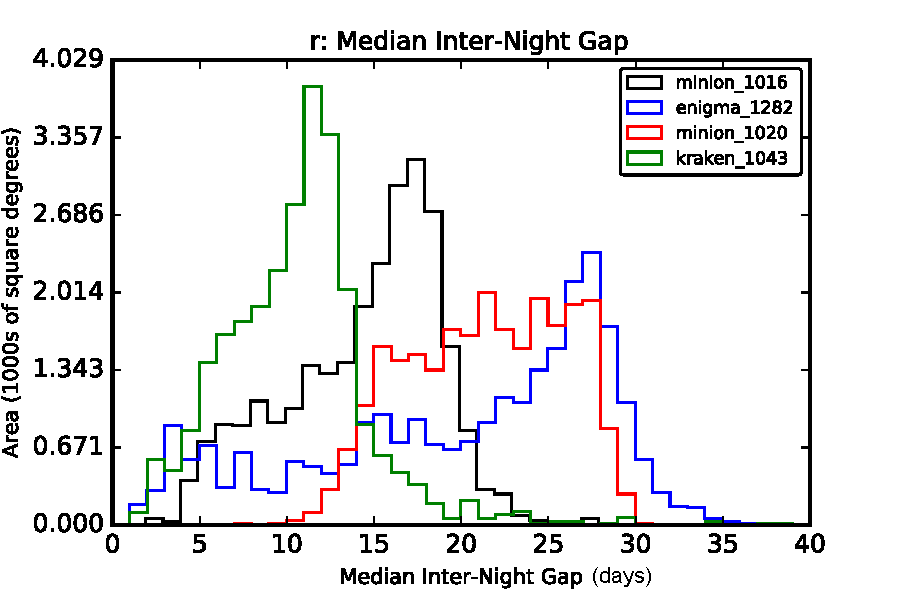
\includegraphics[width=0.45\textwidth]{figs/transients/MedianInter-NightGap_r.pdf}
}
\caption{ Histograms of median $r$-band intra-night visit gaps (hours,
	left) and inter-night visit gaps (days, right)
for several OpSim runs.  Current simulations don't revisit a field in the
	same filter for a period of weeks after a 30-minute visit pair.}
\label{fig:tgaps_r}
\end{figure}

% don't just care about gap between consecutive obs, though; first-last obs
% in a night
\emph{In fact, if the transient community were to design an optimal strategy for short and intermediate duration transients it would likely include 2 visits at a short time interval in different filter, and a third visit at a later time, but within the same night, with one of the two filters already used.}



% --------------------------------------------------------------------

\subsection{Discussion}
\label{sec:\chpname:discussion}

LSST's currently simulated cadences have significant cadence gaps for
timescales between nightly visit pairs and intra-night revisits.  For
many transient science cases, rolling-type cadences that improve the
sampling of a subset of events may be helpful in maximizing the
transient science that can be done with LSST: the minimum lightcurve
sampling required to adequately discover or characterize them may
still be larger than that provided by baseline cadences.  However,
even moderate adjustments (e.g., lengthening the visit pair spacing,
or optimizing the deep drilling filter strategy) may yield
improvements.


The metrics presented in these sections are initial efforts towards
quantifying these goals, and they suggest specific directions for new
OpSIM experiments.  More detailed efforts to understand and model the
challenging problem of transient classification with sparse
lightcurves will be needed in order to best guide LSST's time-domain
observing strategy.

\navigationbar

% --------------------------------------------------------------------


% SECTION:
%    transient.tex
%
% CHAPTER:
%    transients.tex
%
% ELEVATOR PITCH:
%    Explain in a few sentences what the relevant discovery or
%    measurement is going to be discussed, and what will be important
%    about it. This is for the browsing reader to get a quick feel
%    for what this section is about.
%
% COMMENTS:
%
%
% BUGS:
%
%
% AUTHORS:
%  Stefano Valenti , Federica Bianco (@fedhere)
%
% ====================================================================

\section{Realtime Identification of Young Transients}
\def\secname{\chpname:transientsAge}\label{sec:\secname}


\credit{svalenti}, \credit{fedhere} % (Writing team)

For many transients, the first few hours after event beginning reveal a tremendous amount of fundamental information. A large number of resources in the transient community are devoted to the study of the very early phases of transients (e.g. SNe, GRBs). Since real-time discrimination is a very hard task, it is then important to be able to select, among the large number of transients discovered by LSST, the youngest objects, in order to devise follow-up plans and best distribute precious follow-up resources. In this section we investigate the feasibility of identification of young transients (identified within few hours after the event occurs) from the LSST data alone, using the intra-night visits.

The Baseline Cadence~\opsimdbref{db:baseCadence} predicts that, on average,
fields in the main survey are revisited every $\sim3$ days in any filter
(\autoref{fig:enigmaGapAll}), and every $\sim15$ days when using only
$r$ band visits (\autoref{fig:enigmaGapr}).  Hence, we are most likely
to discover faint transients that are within 3 days of peak brightness.
However, for the small subset of nearby events, we can hope to discover
them within a few days of explosion.  The challenge is to discriminate
these truly young events from newly-discovered SN that are near peak
brightness.
Within the~\opsimdbref{db:baseCadence} cadence, and most cadences
realized thus far, the second intra-night visit occurs around 30 minutes (left panel of \autoref{fig:tgaps_r}).
after the first visit (to maximize the Solar System moving objects recovery,~\autoref{chp:solarsystem}). We want to understand {\emph{how the intra-night gap enables, affects, and can be used to maximize the identification of new transients as young}}, where, by young, we mean within a day of outburst/explosion.

To begin to answer this question, we limit our investigation to light curve shape in just the $r$ band, and specifically to what can be done in $r$ band. We have selected a representative set of transients with good photometric coverage in the first week after the the outburst/explosion (left panel of \autoref{fig:earlyslope}) and computed the light curve slope as a function of time in magnitudes per day (right panel of \autoref{fig:earlyslope}). In \autoref{fig:earlyrise} we report the change in $r$ brightness between the first and the second visit for the same set of transients as function of phase. The similarity matrices in \autoref{fig:simmatrix} represent the distance in this quantity for each transient pair for time gaps between observations ranging between 30 minutes and 24 hours.

Despite the heterogeneity in light curve shapes, most of the transients show a similar change in brightness on short time scales.
This confirms that early classification of the transient sub-type is a
major challenge. However, since in general young transients show a fast
increase in brightness, it is much easier to assess whether a transient is
\emph{young}.  Simply put, young transients will show a much larger
brightness change between visits than old events.
This discrimination is aided by a larger time gap between visits (e.g. 2 hours).
Within 30 minutes the change in brightness is of the order of $1\%$, or
even less, for most transients even within the first $\sim3$ days from the
start of the outburst/explosion (\autoref{fig:earlyslope}, left). Thus a
measurement of the change would require a $SNR\gtrsim500$ on each
measurement. Longer gaps give us more leverage: with a time gap of
$\sim2$~hours after the first visit, the change of brightness will increase
to $\sim5\%$. However the breadth of the gap is not unlimited: a gap of 24
hours imposes a significant delay in triggering follow up for these
fast-evolving events.

A natural metric to compare cadences for this purpose
is the median time difference between
the first and last observations of a field each night.  This differs from
the \MAFmetric{IntraNightGapsMetric}, as the latter only compares consecutive
observations of a field and hence underestimates the nightly time baseline
when there are three or more observations of a field in a night.

The classification of interesting transients, at an early stage, can be
aided by using supplementary information, such as historical information
from previous visits, and by color information about the transient. But to
properly assess the color of an evolving transient, the
gap between observations in different filters should not exceed a few hours
(\autoref{sec:\chpname:SNtransients}).

Finally, we stress that the quality and completeness of early
multiwavelengh data available at this time is limited. The sample of
astronomical transients used here is not comprehensive, and a uniform
set of homogeneous data of different transients is still needed in
order to further investigate the ideal separation between
observations, the need for color information, and the tension between
the two.

{\emph{In the light of these considerations, we recommend the
    simulation of a cadence with three visits per field, per night,
    two in the same band, but spaced by two hours or more, and a third
    in a different band. This criteria could be limited to the
    extragalactic sky, away from both the ecliptic plane and the
    galactic plane, where recovery of Solar System objects puts less
    strain on the cadence requirements.  The current 3-visit \OpSim run
    (\opsimdbref{db:NEOswithVisitTriplets}) is inadequate since it
    does not include the constraint of one visit being in a different
    filter.}}

{\emph{Furthermore, we note that the currently envisioned deep
    drilling cadence prioritizes depth per visit at the expense of a
    higher cadence. One hour per night on a deep drilling field
    reaches a depth that not required for almost all transient science
    cases, and by cycling to a different field each night, the time
    between visits for a particular field (4-5 days) is too long for
    many important science cases. Even with higher overhead, a more
    useful approach for nearly all transient science, that the deep
    drilling fields are designed to facilitate, would be to observe
    three or four of the available fields each night for 15 or 20
    minutes.}}

\begin{figure}[hbt]
\centerline{
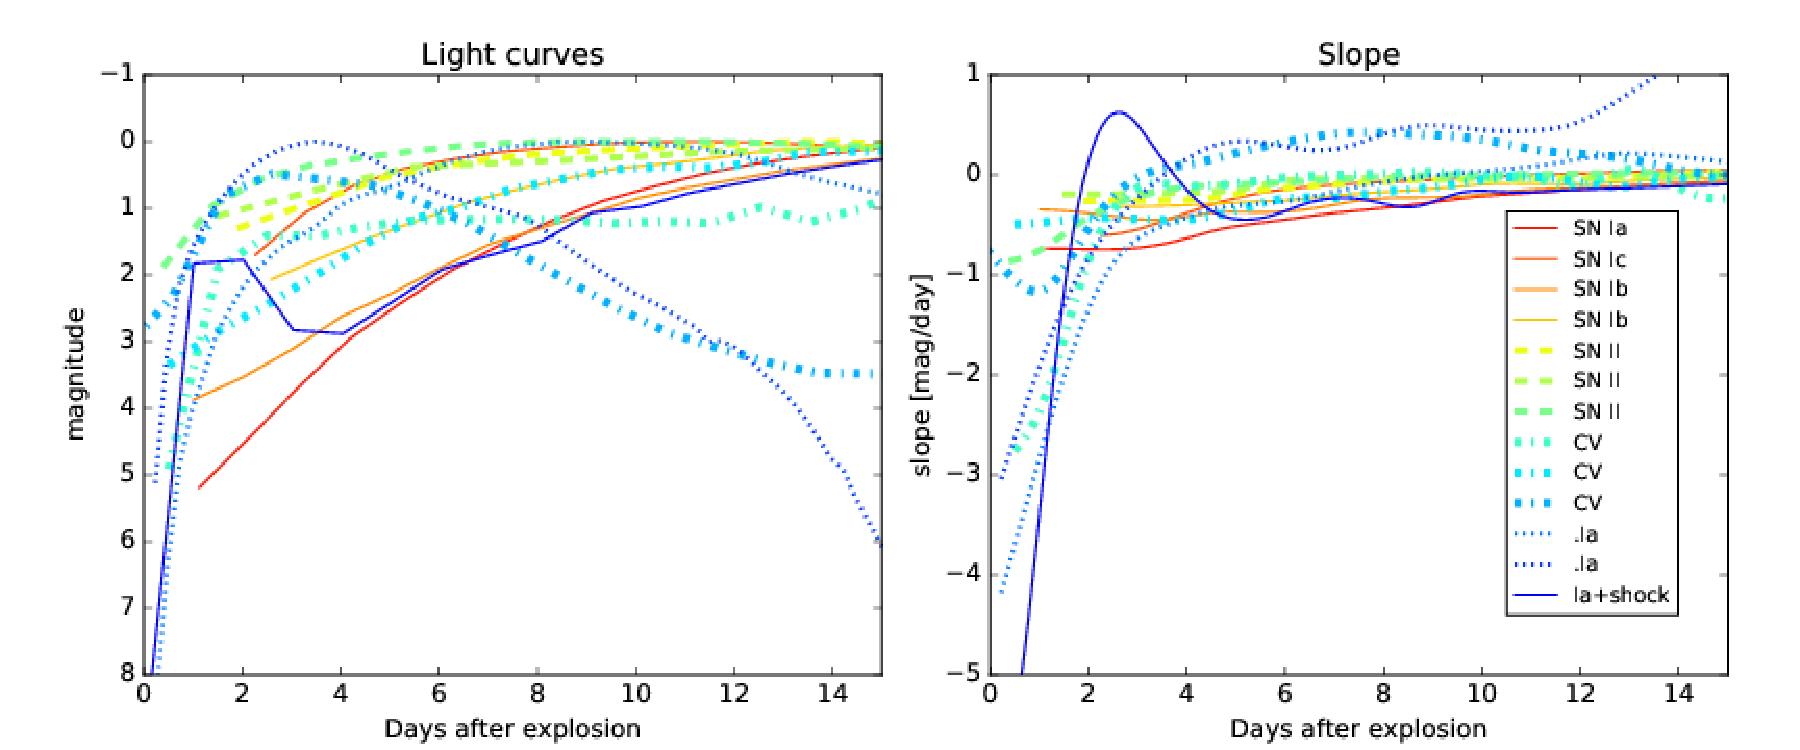
\includegraphics[width=\textwidth]{figs/transients/earlyslope1.pdf}
}
\caption{\emph{Left}: $r'$-band light curve for representative transients as function of the phase from the beginning of the transient outburst/explosion for the first few days of the transient life. \emph{Right}: slope of the transient evolution. Data from: SN~Ia,~\citet{Olling15}; SNII,~\citet{Rubin16}; SN~.Ia,~\citet{Shen10}; SN~Ib,~\citet{Valenti11},~\citet{Cao13}; SN~Ic,~\citet{Mazzali02}; CV, ~\citet{Sokoloski13}, Finzell et al. (in prep), SN~Ia+interaction (see~\autoref{sec:\chpname:SNtransients}).}
\label{fig:earlyslope}
\end{figure}

\begin{figure}[hbt]
\centerline{
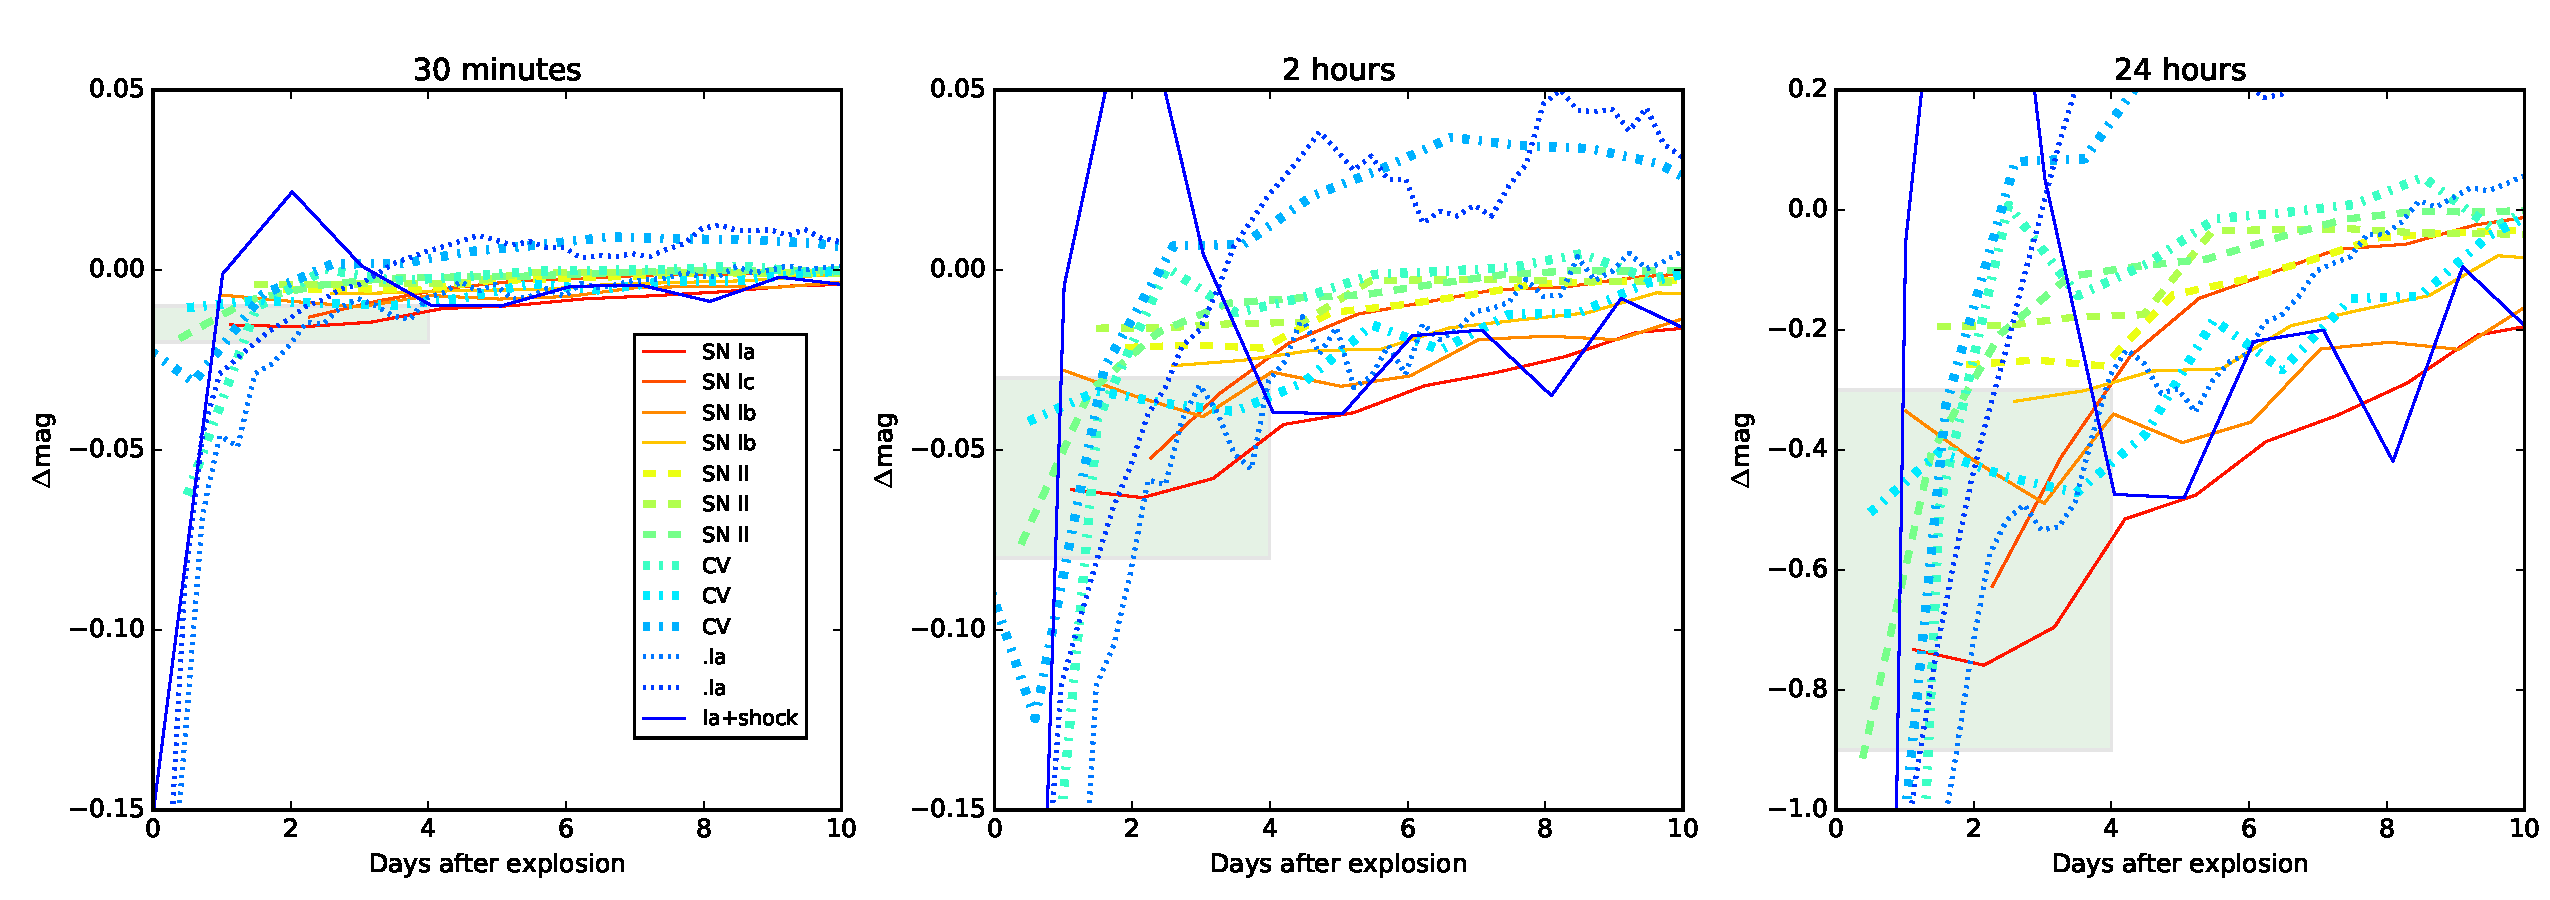
\includegraphics[width=\textwidth]{figs/transients/earlyrise1.pdf}
}
\caption{Observed magnitude change between two consecutive observations for a representative set of astronomical transients, as a function of the phase. We consider observation gaps of 30 minutes  (left panel), 2 hours (central panel) and 24 hours (right panel).
}
\label{fig:earlyrise}
\end{figure}
\begin{figure}[hbt]
\centering
    \begin{subfigure}[t]{0.45\textwidth}
        \centering
        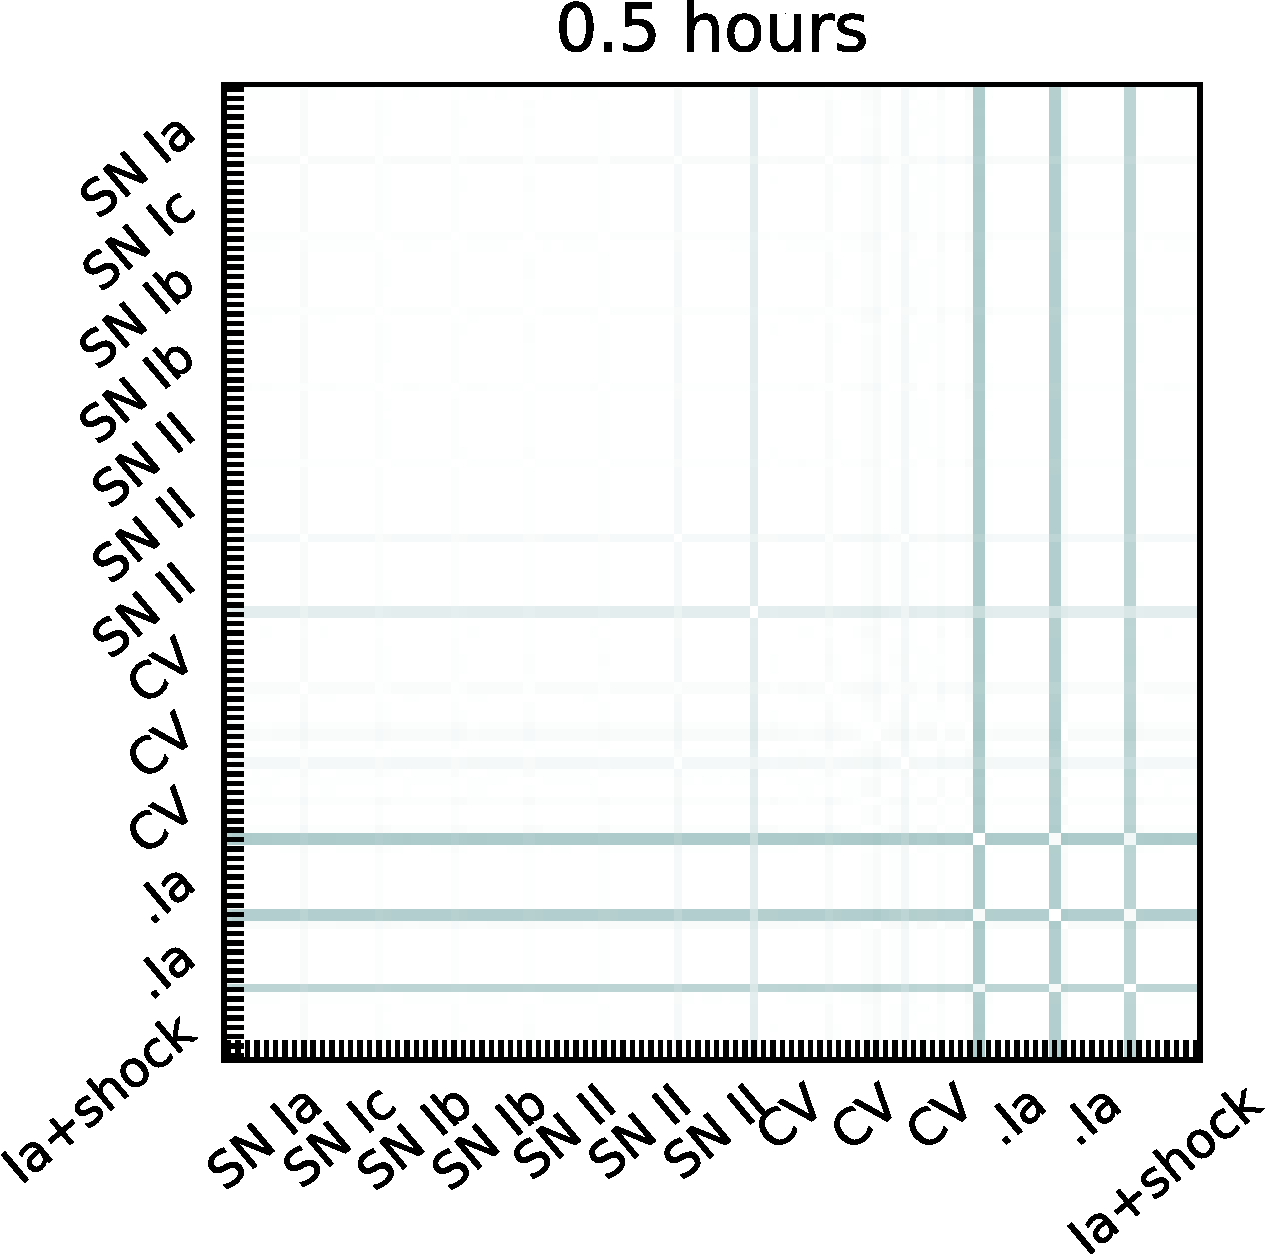
\includegraphics[width=0.8\textwidth]{figs/transients/TransientsAgeSimilarity1.pdf}
    \end{subfigure}%
    ~
    \begin{subfigure}[t]{0.45\textwidth}
        \centering
        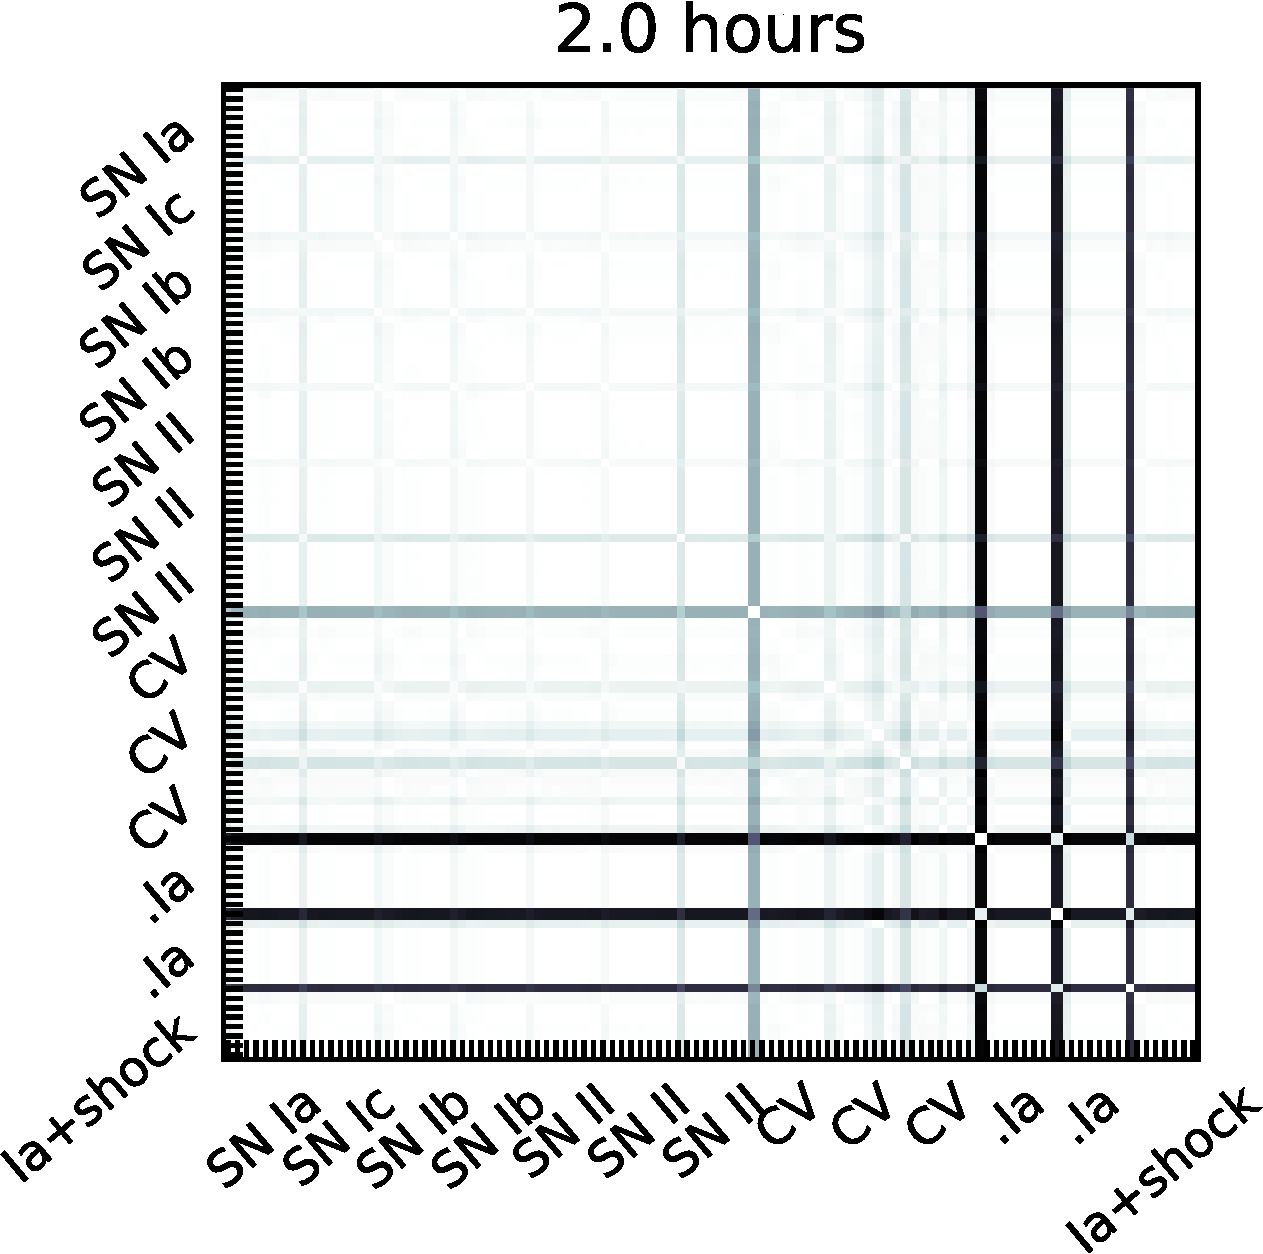
\includegraphics[width=0.8\textwidth]{figs/transients/TransientsAgeSimilarity2.pdf}
    \end{subfigure}


    \begin{subfigure}[t]{0.45\textwidth}
        \centering
        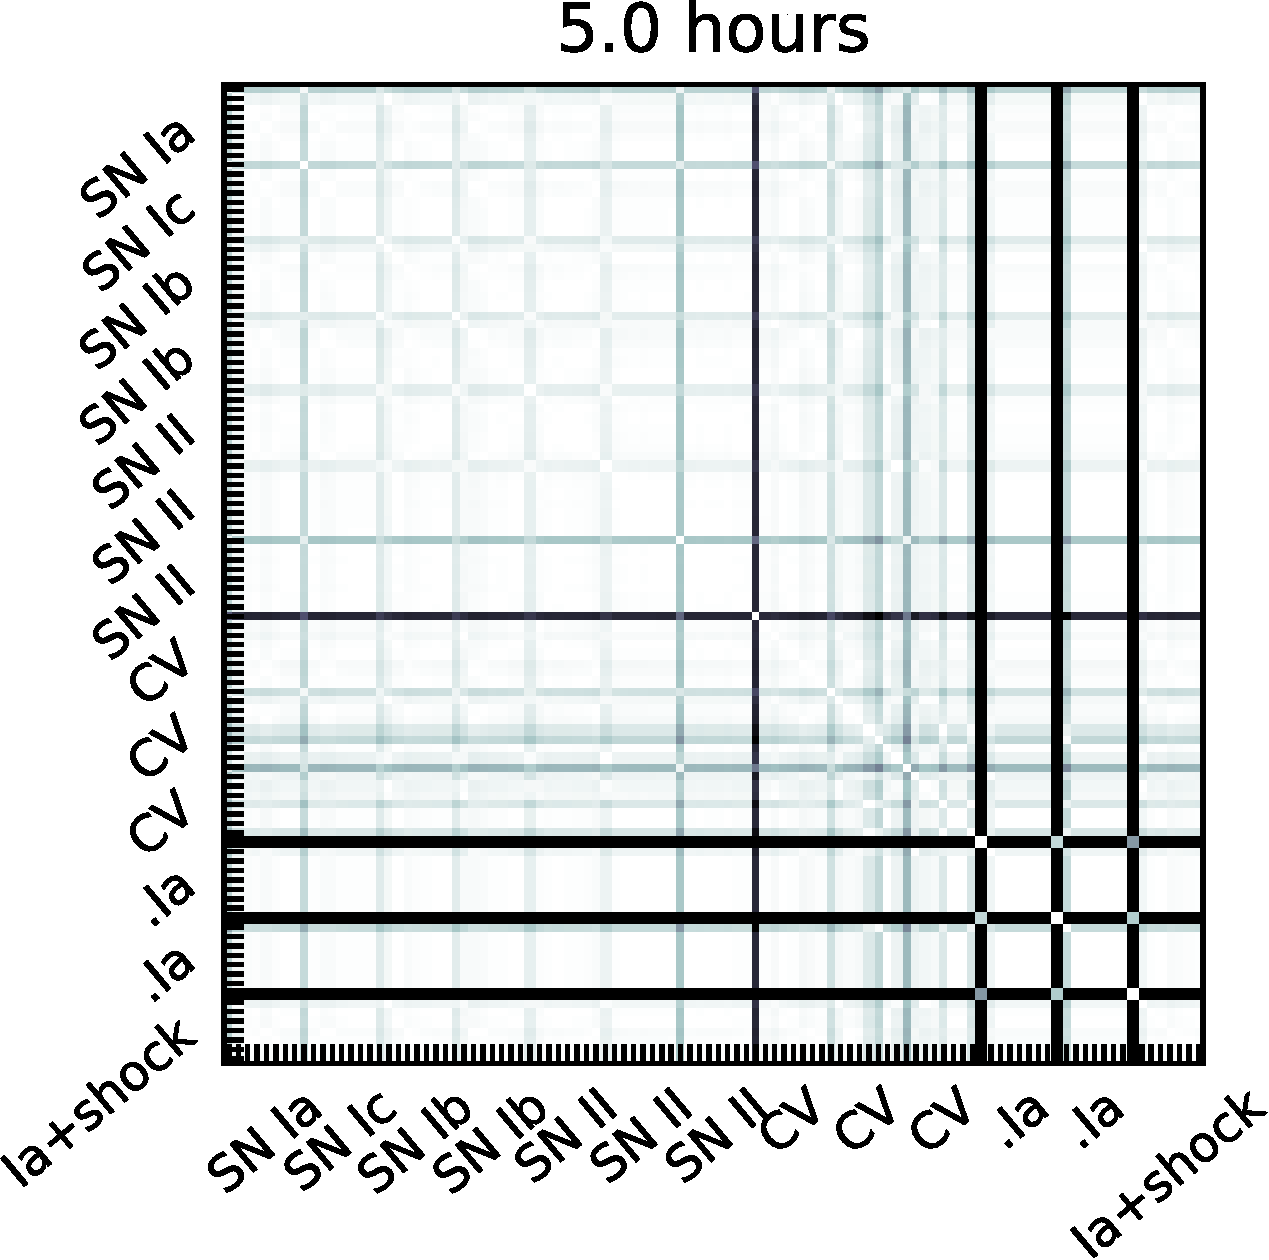
\includegraphics[width=0.8\textwidth]{figs/transients/TransientsAgeSimilarity3.pdf}
    \end{subfigure}%
    ~
    \begin{subfigure}[t]{0.45\textwidth}
        \centering
        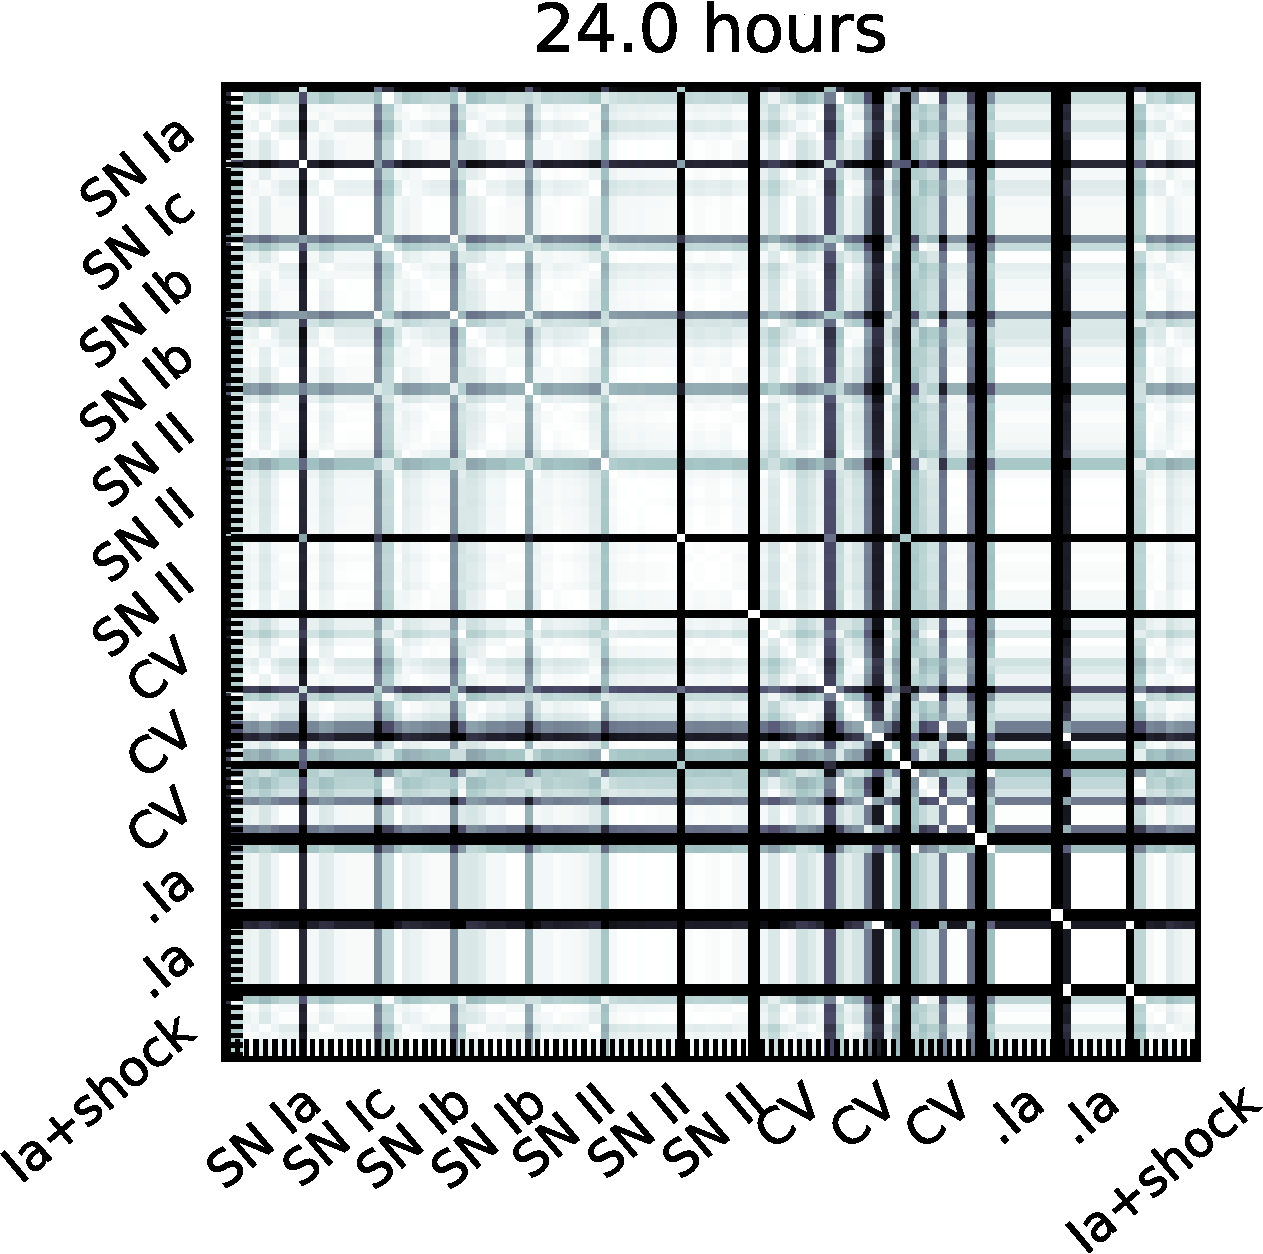
\includegraphics[width=0.8\textwidth]{figs/transients/TransientsAgeSimilarity4.pdf}
    \end{subfigure}

%  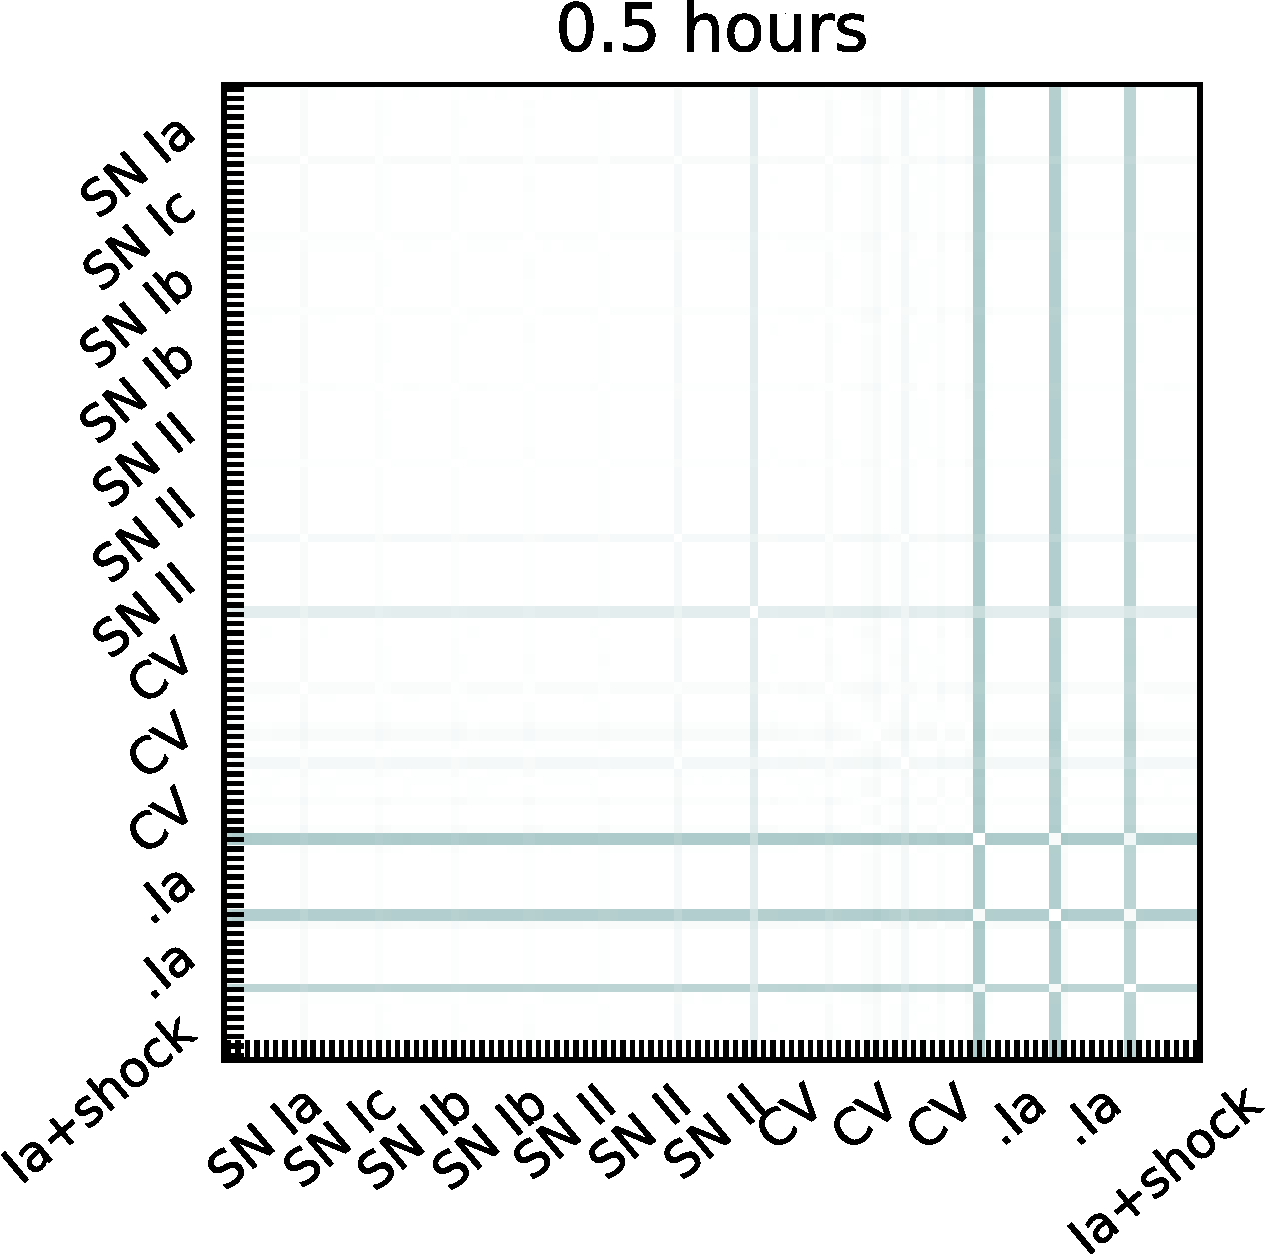
\includegraphics[width=\textwidth]{figs/transients/TransientsAgeSimilarity1.pdf}{figs/transients/TransientsAgeSimilarity2.pdf}

    %  \includegraphics[width=\textwidth]{figs/transients/TransientsAgeSimilarit3.pdf}{figs/transients/TransientsAgeSimilarity4.pdf}


    \caption{Similarity matrix of the transients in \autoref{fig:earlyslope} and \autoref{fig:earlyrise} in $r$ filter for time gaps (starting with the top left panel) of  0.5, 2, 5, and 24 hours.  The similarity is measured as the Euclidean distance between the magnitude change of each transient's pair and it is represented in log scale, with darker colors indicating a larger distance (to a maximum difference $\lvert{\Delta\mathrm{Mag}_1 - \Delta\mathrm{Mag}_2}\rvert ~\sim~8$). For each transient's pair the similarity is calculated for 8 phases within the life of the transients, with the first observation starting at explosion, and as late as 3.5 days after explosion, in 12 hour increments, thus 8 values are associated to each transient pair (as indicated by the tick markers).}
  \label{fig:simmatrix}
\end{figure}

% ====================================================================

 \subsection{Conclusions}

 Here we answer the ten questions posed in
 \autoref{sec:intro:evaluation:caseConclusions}:

 \begin{description}

 \item[Q1:] {\it Does the science case place any constraints on the
 tradeoff between the sky coverage and coadded depth? For example, should
 the sky coverage be maximized (to $\sim$30,000 deg$^2$, as e.g., in
 Pan-STARRS) or the number of detected galaxies (the current baseline
 of 18,000 deg$^2$)?}

 \item[A1:] No strong constraint, as long as larger sky coverage does not compete with dense cadences
required for fast transients.

 \item[Q2:] {\it Does the science case place any constraints on the
 tradeoff between uniformity of sampling and frequency of  sampling? For
 example, a rolling cadence can provide enhanced sample rates over a part
 of the survey or the entire survey for a designated time at the cost of
 reduced sample rate the rest of the time (while maintaining the nominal
 total visit counts).}

 \item[A2:] Frequency of sampling is far more important than uniformity of sampling for early classification of interesting cadence. The rolling cadence is definitely the first step to take, but it is still not enough to identify young transients. A longer than .4 hours intra-night gap or, even better a one day cadence would allow young transients to vary enough to be identified. If the second visit occurs on 0.4-hour time scale, a different filter would be preferred (color information can be alternatively used to identify young transients)


 \item[Q3:] {\it Does the science case place any constraints on the
 tradeoff between the single-visit depth and the number of visits
 (especially in the $u$-band where longer exposures would minimize the
 impact of the readout noise)?}

 \item[A3:] Anything that reduces the number of visits per field potentially compromises the objectives.

 \item[Q4:] {\it Does the science case place any constraints on the
 Galactic plane coverage (spatial coverage, temporal sampling, visits per
 band)?}

 \item[A4:] The requirement for multiple visits/filters per night applies to all fields.

 \item[Q5:] {\it Does the science case place any constraints on the
 fraction of observing time allocated to each band?}

 \item[A5:] No.

 \item[Q6:] {\it Does the science case place any constraints on the
 cadence for deep drilling fields?}

 \item[A6:] As discussed in detail above, short bursts of visits separated by several days is not
satisfactory - deep drilling cadences can be devised to provide excellent sampling.

 \item[Q7:] {\it Assuming two visits per night, would the science case
 benefit if they are obtained in the same band or not?}

 \item[A7:] If two visits only, different filters may be the most effective. If more than two visits, the most closely spaced pair should be in the same filter, and the other visits should include at least one other filter.

 \item[Q8:] {\it Will the case science benefit from a special cadence
 prescription during commissioning or early in the survey, such as:
 acquiring a full 10-year count of visits for a small area (either in all
 the bands or in a  selected set); a greatly enhanced cadence for a small
 area?}

 \item[A8:] A greatly enhanced cadence would provide a strong test of the methodology and would jump-start the science.

 \item[Q9:] {\it Does the science case place any constraints on the
 sampling of observing conditions (e.g., seeing, dark sky, airmass),
 possibly as a function of band, etc.?}

 \item[A9:] None unique to transients.

 \item[Q10:] {\it Does the case have science drivers that would require
 real-time exposure time optimization to obtain nearly constant
 single-visit limiting depth?}

 \item[A10:] No.

 \end{description}

 \navigationbar


% --------------------------------------------------------------------

% ====================================================================
%+
% SECTION:
%    sn.tex
%
% CHAPTER:
%    transients.tex
%
% ELEVATOR PITCH:
%
%-
% ====================================================================

\section{Supernovae as Transients}
\def\secname{\chpname:SNtransients}\label{sec:\secname}

\credit{fedhere}

Supernovae (SNe) represent the final dramatic stages of the life of many
stars. The term SN covers a diverse set of phenomena: explosion of
low mass stars in binary systems, thermonuclear SN or SN Ia (also
discussed in \autoref{sec:supernovae}), explosions of high mass stars,
core collapse (CC) SNe, and even terminal explosions of more exotic
systems, yet to be understood, like Super Luminous SNe
(SLSNe). Phenomenologically, the observables of the explosion are
also diverse. The transient duration ranges from weeks to
months and even years. The electromagnetic energy radiated ranges between
$\sim0.1$ (faintest CC SNe), to $\sim1$ (SN Ia) and $\sim100$ (SLSNe)
$\times 10^{49}$ erg, corresponding to absolute magnitudes at peak
ranging between $\sim-19$ and $\sim-22$.

LSST's contribution to SNe studies can be substantial. Synoptic
surveys such as SDSS, SNLS, PTF, PanSTARRS have revolutionized our
understanding of SN time and again, exposing their diversity,
and revealing different progenitor channels. LSST's first crucial
input will be discovery: the normal type Ia SN rate out to redshift
$z=1$ is estimated to be $\sim200 ~(\mathrm{sq. deg.})^{-1}$ per
year\footnote{\url{http://www.lsst.org/sites/default/files/docs/Wood-Vasey_086.11.pdf}},
and SN~Ia represent only about 1/4 of all SN
events~\citep{Li11b}: tens of millions of stars will explode
within the LSST footprint every year. The main factors affecting
LSST SN science concern:
\begin{enumerate}
\item
LSST's SN discovery power,
\item
LSST's discrimination power,
\item
the quality of the statistical sample over time.
\end{enumerate}
Items 1 and 2 are \emph{time sensitive}, while the latter
is not, although it is interesting to understand the pace at which a
science question can be advanced in the lifetime of LSST.

{\bf \emph{Discovery:}} the SN~Ia discovery is rate is a standard LSST time-domain metric: a
fraction of $\sim40\%$ SN~Ia $z\lesssim0.5$ are expected to be discovered pre-peak
luminosity within the standard LSST survey
(e.g. \opsimdbref{db:baseCadence}~Figure~\ref{fig:enigmaEarlySNe}). The
topic of SNe discovery is discussed in further detail in
\autoref{sec:supernovae}.

The next step is then {\emph{discrimination}}, and the question we need
to answer, for SNe as well as for most other transients, is: will LSST
photometry allow us to distinguish SN from other transients, and to
distinguish the different types of SN? And further: will this be
achievable in time to appropriately direct follow-up efforts? This is
particularly difficult considering that photometric classification
schemes have only achieved modest performances in distinguishing, for
example, SN~Ic from SN~Ia.

When a large statistical sample of SNe is generated, LSST's photometry
may allow setting constraints on the diversity of the sample, even as a
standalone survey, without the aid of follow-up efforts.  {\emph Thus
  LSST \bf{alone} can shed light on the diversity within the
  population of SN}, which in turn may constrain the genesis of the
explosion.\footnote{Reliable typing of a SN and redshift determination
  would still require auxiliary data.} For SN~Ia, where the exploding
star is a carbon-oxygen White Dwarf (WD), a major outstanding question
that can be answered by an LSST photometric sample is
what is the percentage of SN Ia that arise from a
\emph{double-degenerate} (DD) progenitor system (a carbon-oxygen WD-WD
binary), from a \emph {single-degenerate} (SD) system (a WD-Main Sequence
 or WD-Red Giant (RG) binary), or from a \emph{merger} (a WD-WD
 binary with a He and a carbon-oxygen WD).
 Answering this question would reduce the
scatter in the Hubble diagram if SNe from different progenitors are
shown to require different standardization~\citep{Scolnic2014}. On the
CC~SN side: the diversity of SN sub-classes, and the relationship
between them (is there a phenomenological continuum or are they actually
distinct classes, e.g. between IIp and IIL, or Ib and IIb?) is yet to
be understood. Exceptionally well-studied objects may answer these
questions: individual SN Ia with tight constraints on the progenitor
system show, for example, that both single and double degenerate
progenitors exist (e.g. SN 2011fe, \citealt{Li11}, ~\citealt{Olling15}
and PTF 11kx, \citealt{Dilday12}). However, a statistical sample is
needed to set constraints on populations~\citep{Hayden2010, Bianco11}.

Thus the technical question to be answered is: how much detail can be
sacrificed in favor of sample size without compromising diagnostic
power? And the diagnostic power relies on color and sampling: thus
what is the trade-off between cadence in the same filter, and
observations in different filters. Specifically, transients can be
distinguished early from two photometric characteristics: rise time
and color. There is a tension between these observables, as discussed
in Section~\ref{sec:\chpname:transientsAge}. Obtaining colors relies
of course on obtaining photometry in different bands as close as
possible to \emph{simultaneously}.  However, assessing the rise slope
is best done with a single filter, so prompt characterization also
needs multiple epochs within a night, although separated by at least a
few hours, in the same filter, as observing with different
filters it is impossible (or very hard) to separate shape from
color. Colors are an important diagnostic for the
statistical sample: as long as the epoch of peak is reliably assessed
coadded light curves can be studied, which is the goal of the analysis
that follows.

\subsection{Distinguishing progenitor scenarios}

In this chapter we envision and design a SN related metric that works
on a large sample (months-to-years of LSST data) and assesses the
ability to characterize the contribution of SNe with specific features
to the global population: as a test case we will use the identification of
an early blue excess for SN type Ia, a signature of interaction with a
companion, and thus of a SD progenitor. Equivalently, the presence of
an early blue excess in CC~SNe could be the signature of
shock breakout which directly measures the radius of the progenitor
star. We perform the simulation on SN~Ia since statistical studies of
samples that set constraints on progenitor fractions (fraction of DD
vs SD progenitors) exist and can be used as a
benchmark~\citep{Hayden2010, Bianco11}.  What we evaluate as a
\emph{figure of merit} (FoM) for this science deviates from the
guidelines for figures of merit, since LSST will surely be able to
answer this question \emph{at some point} and we measure \emph{how
  fast} LSST can answer this question. Our FoM is time
within the survey required to achieve a sufficiently large sample of
SNe to enable us to distinguish
populations with different contribution from DD and SD progenitors.
We rely on simulations of the observables of the population for
different sample sizes, and on the \MAFmetric{transientAsciiMetric} to
determine the detectability of interacting vs non-interacting
SNe. We are developing a metric (\texttt{colorGapMetric}) to assess
the gap between of detections in 2 filters. In the meantime, we rely on
the estimated of the gap between observations in a single filter, and
in any filters (see~\autoref{sec:\chpname:analysis}).

We simulate interacting SNe from the Nugent templates \citep{Nugent02}
injecting the angle-dependent effects of interaction with a companion
as simulated by \citep{Kasen10}, for a $2~M_\odot$ and a $6~M_\odot$
MS companion stars, and a $1~M_\odot$ RG companion, following the
procedure designed in ~\citep{Bianco11}. We create synthetic progenitor
populations with a fraction of single degenerate progenitor systems
$0.05 \leq f_\mathrm{SD} \leq 0.6 $ in 0.05 intervals, and random lines of
sight with respect to the binary's geometry. One such lightcurve, with
maximal interaction effects, is shown in \autoref{fig:kasenlc}, also
indicating how it may be observed by LSST. For each population, we
simulate the observation of colors by selecting random epochs with a
granularity of 1 day within the first 10 days after explosion, and
subtracting the magnitude in different filters at the same epoch
$\pm~1$~day for each SN, and we include the effects of observational
noise by generating datapoints from a draw within a Gaussian
distribution centered at the color measured in the previous step and
with standard deviation $\sigma_\mathrm{pop} = 0.1$, 0.3, and 0.5.
The SNR requirement is
translated into a requirement on each
observation of $\mathrm{SNR} >
\frac{1.0}{\sqrt{2.0}~\sigma_\mathrm{pop}}$.
We generate populations of $N_\mathrm{pop}=100$,~1000,~10000 $z~=~0.5$ SNe,
observed in $g'-r'$, as a representative case. Because the effect is
heavily chromatic and becomes essentially negligible
by $r$ band, $u'-i'$ gives the most leverage. However $g'$ and $r'$
are the best observed LSST bands in most cadences. An extension of
this work should then consider $g'-r'$, $u'-r'$, $g'-i'$, and $u'-i'$.

\begin{figure}[hbt]
\centerline{
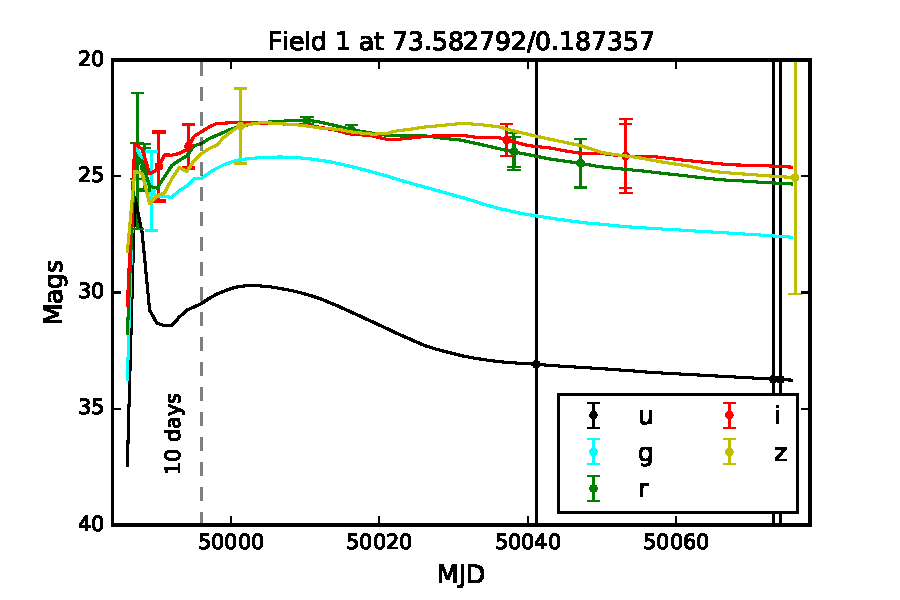
\includegraphics[width=0.6\textwidth]{figs/transients/LSST_Kasen_lcv0.pdf}
}
\caption{ A normal SN Ia lightcure at z=0.5 showing interaction with a
  RG companion as seen from the most favorable viewing angle: the
  effect of interaction as simulated by \citet{Kasen10} is added on
  top of a lightcurve simulated from the \citealt{Nugent02}
  templates. The data points represent one possible set of LSST
  observations of this transient, obtained by running the
  \MAFmetric{transientAsciiMetric}.  This particular event is detected in
  $g'$, $r'$, and $i'$ within the first 10 days.}
\label{fig:kasenlc}
\end{figure}

We perform Kolmogorov-Smirnoff ($KS$) and Anderson-Darling ($AD$) tests
to evaluate our diagnostic power as a function of sample quality,
$SNR$, and sample size, $N_\mathrm{pop}$.  In
\autoref{tab:SNprogenitors} we report the ability to distinguish a
population with a $f_\mathrm{SD} > x$ from $f_\mathrm{SD}=0.05$; \emph{the
number reported is the SN~Ia fraction from SD progenitors that can be
distinguished at a $p\mathrm{-value}~\leq ~0.05$}.

\begin{table}
\begin{center}
  %\begin{tabular}{ c | c| c| c | c | c| c| c | }
  \begin{tabular}{ c | c| c| c |  }
$g-r$&\bf{$N_\mathrm{pop}$=100}&\bf{$N_\mathrm{pop}$=1,000}&\bf{$N_\mathrm{pop}$=10,000}\\%& $g-i$&\bf{$N$=100}&\bf{$N$=1,000}&\bf{$N$=10,000} \\
  \hline
  {\bf $\mathrm{SNR}~\geq~1.4$}&  -  & 0.2 & 0.1 \\%& &  -  & -  &  0.2 \\
  {\bf $\mathrm{SNR}~\geq~2.0$}&  - & 0.2 & 0.1 \\%& &  -  & 0.2 & 0.1 \\
  {\bf $\mathrm{SNR}~\geq~7.0$}& 0.2 & 0.1 & 0.1 \\%& & 0.4 & 0.1 & 0.1 \\
%&&&&&&&\\ $u-i$&\bf{$N$=100}&\bf{$N$=1,000}&\bf{$N$=10,000} & $u-r$&\bf{$N$=100}&\bf{$N$=1,000}&\bf{$N$=10,000}\\
% \bf{$\sigma_\mathrm{pop} = 2.0$}&  -  & -  &  0.2 & &  -  & -  &  0.2 \\
% \bf{$\sigma_\mathrm{pop} = 1.0$}&  -  & 0.2 & 0.1 & &  -  & 0.2 & 0.1 \\
% \bf{$\sigma_\mathrm{pop} = 0.5$}& 0.4 & 0.1 & 0.1 & & 0.4 & 0.1 & 0.1 \\

 \hline
  \end{tabular}
  \caption{Minimum fraction of single-degenerate (SD) SN~Ia in a sample of size $N_\mathrm{pop}$ of $z~=~0.5$ SNe that can be distinguished from a population with a fraction of 0.95 double-degenerate (DD) and 0.05 SD SNe~Ia, for a given quality cut on each observed datapoint ($\sigma_\mathrm{pop}$).}
\label{tab:SNprogenitors}
\end{center}
\end{table}

Now we can evaluate how long it will take for a given LSST
cadence to obtain a sufficient number of observations in the 2 desired
bands, separated by less than 1 day, that pass the SNR requirements.
This should be done in a full Monte Carlo simulation, injecting
light curves with the proper light curve shape at the proper rate.  Note
that, because the early light curves of interacting SD SN~Ia are
brighter, they should be more easily detected. However, at this stage we
can take some shortcuts. \emph{First shortcut}: we evaluate the
relative observability of SNe with excess, and SNe without excess at
$z~=~0.5$ and adjust the number of detections according to
the injected ratio.  The relative detectability can be assessed with
the \MAFmetric{transientAsciiMetric}, which allows us to see how OpSim
recovers observations of transients with realistic shapes. We conclude
that for RG-WD progenitors the detectability is enhanced by $\sim50\%$ in
 $g'$ compared to SD progenitors, and slightly less in $r'$.
Then we extract from the \MAFmetric{transientAsciiMetric}, the number of
\emph{color observations}, i.e. observations in 2 bands within 1 day
of each other, each fulfilling our SNR requirement for the color for
3-, 6-, and 12 months of survey in year 1.

With the goal of distinguishing a SD contribution of 10\% to the SN Ia
population from a 5\% contribution to a three-sigma level ($p$-value
$<0.05$) we need more than 1000 detections within 1 day in 2 filters
at a $\mathrm{SNR}~\geq~7$: \autoref{tab:SNprogenitors}. But the pairs
of observations we recovered in the previous steps are within the
first 10 days but with any gap in time. \emph{Second shortcut}: To
include the constraint that the detections should be within 24 hours
we use to the \MAFmetric{InterNightGapsMetric}, which is plotted in
~\autoref{fig:enigmaGapAll}.  For the \opsimdbref{db:baseCadence} we
estimate $~\sim10\%$ of the observation are revisited within a
night. With the assumption that this is likely to happen in two
different filters, which is \emph{non-conservative}, but neglecting
intra-night observations that may happen in the two different filters,
which is a \emph{conservative} assumption our numbers drop by a factor
10. The lightcurves are injected with an event rate designed to be
consistent with the discovery rate measured in \ref{sec:supernovae}.

With all these assumptions standing, we find that that only 3 months
of survey are sufficient to provide a sufficiently large and
sufficiently high SNR sample for our purpose, and improve on the
findings on this topic that were achieved with
SDSS~II~\citep{Hayden2010}, and 3 years of SNLS data~\citep{Bianco11}
with \opsimdbref{db:baseCadence} or the
\opsimdbref{db:NEOswithVisitTriplets}. The
\opsimdbref{db:NEOswithVisitTriplets} requires three visits, thus
increasing the timeline for inter-night observations. Although it does not
require the observations to be in any specific filters, and with the
addition of the third visit within the same night, it increases the
typical intra-night gap, it outperforms \opsimdbref{db:baseCadence} slightly.
It is possible that a detailed investigation
of the true \emph{inter-night gap between different filters}, or the
addition of a requirement in the cadence that one of the night filters
be different than the others (possibly requiring an increased gap
between two of the three images to minimize filter changes) would
provide valuable data for this kind of studies even faster.

\emph{This exercise demonstrates the power of LSST in collecting large high SNR samples of transients, but we must remind the reader that these conclusions, and generally large sample analysis, rely on having properly identified both the transient class (normal SN~Ia) and the date of maximum! This, once more, highlights the importance of prompt identification and classification: for SN~Ia this likely will limit this work to objects that could be identified spectroscopically, enhancing the importance of follow-up.}


\autoref{fig:sndetect} shows the detection rate for SN~Ia at $z=0.5$
in absence of shock interaction as a function of SNR (obtained by summing in quadrature the errors on $g'$
and $r'$) for 3, 6 months, and a year of
\opsimdbref{db:baseCadence} and \opsimdbref{db:NEOswithVisitTriplets}.
% (ideally I will plot it for the other survey as well tonight)



\begin{table}
  \begin{tabular}{l|p{8cm}|c|c|p{3cm}}
    FoM & Brief description & {\rotatebox{90}{\opsimdbref{db:baseCadence}}}
	  & {\rotatebox{90}{\opsimdbref{db:NEOswithVisitTriplets}}} & Notes \\
    \hline
    \thesection-1 & \footnotesize{\texttt{SNIaprojenitorMetric},
    \nolinebreak{\texttt{1,000 detections}}}      & 3 & $<3$ &
    \footnotesize{Time in month to collect 1,000 relevant observations to distinguish a 5\% from a 10\% SD contribution} \\
    \thesection-2     & \footnotesize{\texttt{SNIaprojenitorMetric},
    \texttt{10,000 detections}}      & $>12$ & $>12$ &
    \footnotesize{Time in month to collect 10,000 relevant observations in months  to distinguish a 5\% from a 10\% SD contribution.}\\
\end{tabular}
\caption{FoMs for statistical SN Ia progenitor studies to assess the contribution of SD progenitors to the SN Ia population.
}
\label{tab:SummarySNprojs}
\end{table}

\begin{figure}[hbt]
  \centerline{
    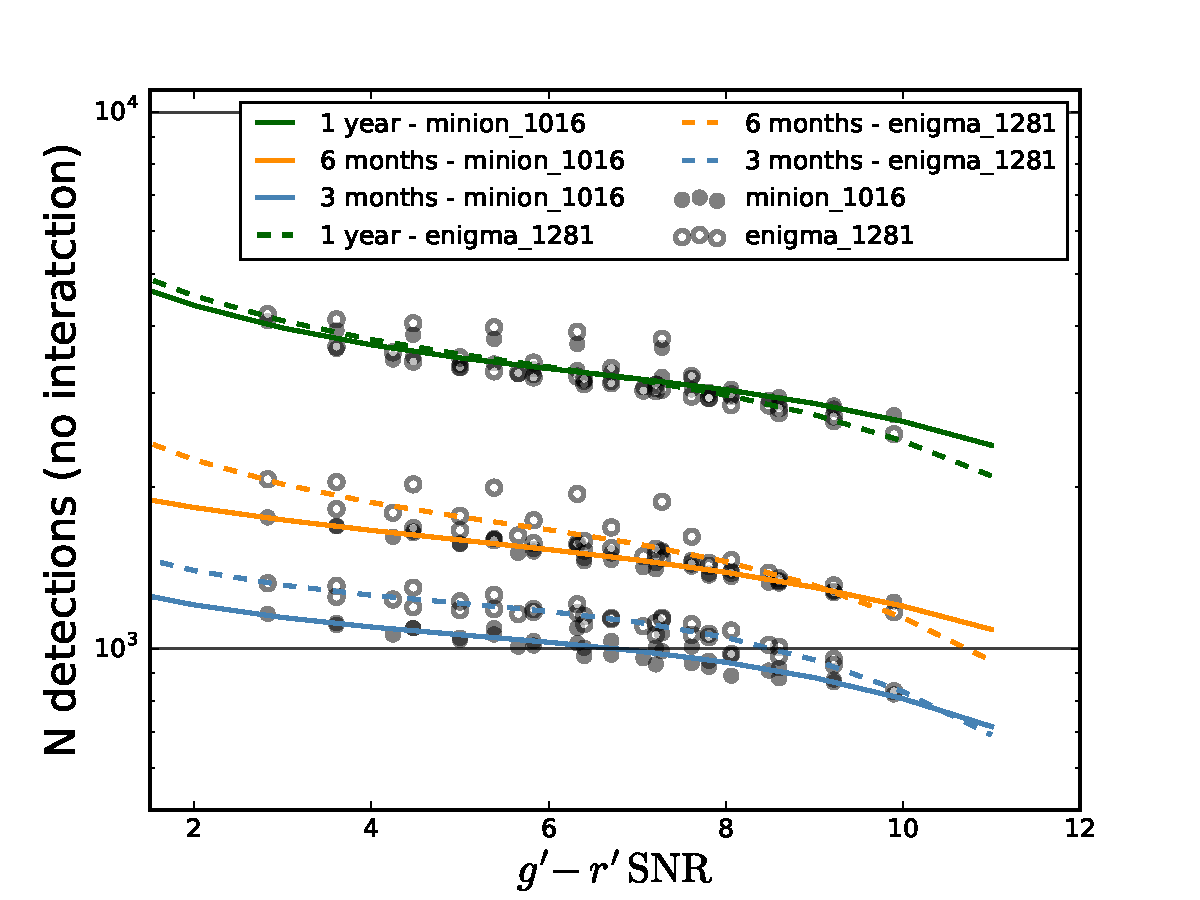
\includegraphics[width=0.6\textwidth]{figs/transients/LSST_Iadetected_wcolor.pdf}
  }
  \caption{
    Normal SN Ia light cure at z=0.5 detected by the \opsimdbref{db:baseCadence} (solid lines) and \opsimdbref{db:NEOswithVisitTriplets} cadence (dashed line) in 3 months, 6 months, and 1 year, that provide color information useful to constrain the progenitor distribution. Line are third-degree polynomial fits.}
  \label{fig:sndetect}
\end{figure}

% ====================================================================
%
 \subsection{Conclusions}

 Here we answer the ten questions posed in
 \autoref{sec:intro:evaluation:caseConclusions}:

 \begin{description}

 \item[Q1:] {\it Does the science case place any constraints on the
 tradeoff between the sky coverage and coadded depth? For example,
 should the sky coverage be maximized (to $\sim$30,000 deg$^2$, as e.g.,
 in Pan-STARRS) or the number of detected galaxies (the current baseline
 but with 18,000 deg$^2$)?}

 \item[A1:] Yes, although this question can be answered with a full simulation that includes a coordinate dependent event rate while the current simulation assumes uniform probability of a transient in the field-of-view and cannot evaluate this trade-off


 \item[Q2:] {\it Does the science case place any constraints on the
 tradeoff between uniformity of sampling and frequency of sampling? For
 example, a rolling cadence can provide enhanced sample rates over a
 part of the survey or the entire survey for a designated time at the
 cost of reduced sample rate the rest of the time (while maintaining the
 nominal total visit counts).}

 \item[A2:] Yes: this science case is sensitive to both. A more sophisticated simulation which also measures the ability to correctly identify the epoch of maximum would be more powerful to answer the question.


 \item[Q3:] {\it Does the science case place any constraints on the
 tradeoff between the single-visit depth and the number of visits
 (especially in the $u$-band where longer exposures would minimize the
 impact of the readout noise)?}

 \item[A3:] Yes, because the diagnostic power depends on both the SNR of each observation and the gap between observations.


 \item[Q4:] {\it Does the science case place any constraints on the
 Galactic plane coverage (spatial coverage, temporal sampling, visits
 per band)?}

 \item[A4:] No.


 \item[Q5:] {\it Does the science case place any constraints on the
 fraction of observing time allocated to each band?}

 \item[A5:] Yes, since it relies on obtaining observations in at least 2 filters.


 \item[Q6:] {\it Does the science case place any constraints on the
 cadence for deep drilling fields?}

 \item[A6:] Yes, although the results have not been analyzed separately for WFD and DD fields.


 \item[Q7:] {\it Assuming two visits per night, would the science case
 benefit if they are obtained in the same band or not?}

 \item[A7:] No. Although  we would benefit greatly from 2 visits in the same filters, and one visit in a different filter to constrain simultaneously shape and color."


 \item[Q8:] {\it Will the case science benefit from a special cadence
 prescription during commissioning or early in the survey, such as:
 acquiring a full 10-year count of visits for a small area (either in
 all the bands or in a  selected set); a greatly enhanced cadence for a
 small area?}

 \item[A8:] A full event rate needs to be included in the simulation to answer this question.


 \item[Q9:] {\it Does the science case place any constraints on the
 sampling of observing conditions (e.g., seeing, dark sky, airmass),
 possibly as a function of band, etc.?}

 \item[A9:] Indirectly, since detection efficiency depends on SNR.


 \item[Q10:] {\it Does the case have science drivers that would require
 real-time exposure time optimization to obtain nearly constant
 single-visit limiting depth?}

 \item[A10:] No.

 \end{description}

 \navigationbar


% --------------------------------------------------------------------

% ====================================================================
%+
% SECTION:
%    grb.tex
%
% CHAPTER:
%    transients.tex
%
% ELEVATOR PITCH:
%-
% ====================================================================

\section{Gamma-Ray Burst Afterglows}
\def\secname{\chpname:grbs}\label{sec:\secname}

\credit{ebellm}

Gamma-ray bursts (GRBs) are relativistic explosions typically classified
by the temporal duration of their initial gamma-ray emission: Long GRBs,
that mark the endpoint of the lives of some massive stars, and short
GRBs, believed to originate from the merger of binary neutron stars. GRB
emission is known to be beamed: the initial prompt gamma-ray emission is
seen only for observers looking at the jet axis. The longer-wavelength
X-ray, optical, and radio afterglow may be seen both by on- and off-axis
observers.  The latter case is known as an orphan afterglow, due to the
absence of gamma-ray emission. On- and off-axis afterglows are predicted
to have different temporal signatures in the optical: On-axis events
decay as a power-law until a jet break, while off-axis events should be
fainter and show an initial rise (Figure \ref{fig:afterglow_lcs}).
Despite systematic searches, no convincing orphan afterglow candidates
have yet been discovered, limiting our knowledge of the beaming fraction
of GRBs and hence their true rates. Well-sampled orphan afterglow
lightcurves would also permit study of the GRB jet structure.

\begin{figure}[hbt]
\centerline{
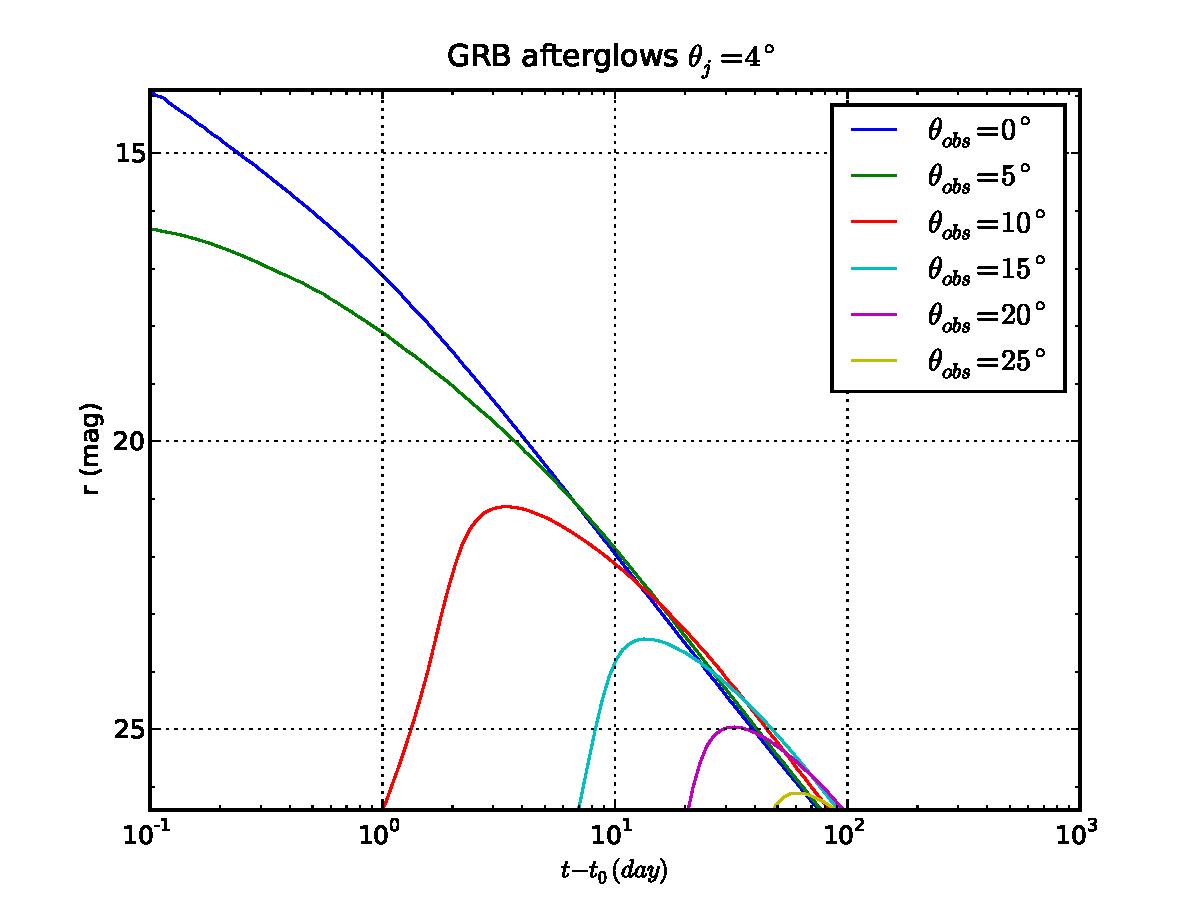
\includegraphics[width=0.6\textwidth]{figs/transients/predicted_afterglow_lcs_mag.pdf}
}
\caption{ Predicted light curves of GRB afterglows by off-axis angle
with respect to the jet axis $\theta_{\rm obs}$ \citep[Figure
8.8,][]{2009arXiv0912.0201L}. The forward shock model is derived from
\citet{2002ApJ...576..120T} and assumes a jet half opening angle
$\theta_j = 4^\circ$, the isotropic equivalent energy of $E_{\rm iso} =
5\times10^{53} \rm erg$, ambient medium density $n = 1$ g cm$^{-3}$, and
the slope of the electron energy distribution $\rm p = 2.1$. The
apparent AB $r$-band magnitudes assume a source redshift $z = 1$. }
\label{fig:afterglow_lcs}
\end{figure}

Because of their rarity, in all but one case \citep{2015ApJ...803L..24C}
to date GRBs have been discovered using their prompt emission by hard
X-ray or gamma-ray all-sky monitors. This selection imposes biases on
the population of relativistic explosions we observe. Baryon-loading in
the GRB jet---a ``dirty fireball'' \citep{2003ApJ...591.1097R}---can
lead to on-axis events without gamma-ray emission.  Only one plausible
candidate has been identified to date \citep{2013ApJ...769..130C}.
Discovery of new dirty fireballs---if distinguished from off-axis
events--would clarify the rates of these events and enhance our
understanding of the diversity of stellar death.

LSST is the survey most capable of resolving these decades-old
questions.  Due to its large aperture and etendue, LSST can detect
faint, fast-fading, and rare cosmological events, potentially enabling
population studies of the high-redshift universe.
\citet{2015A&A...578A..71G} estimated LSST could detect 50 orphan
afterglows each year, more than any other planned survey.

%deep survey helps due to time dilation

%beaming fraction and true rates; jet structure; dirty fireballs?
%GRB-SN connection; probe high-z star formation?

%other fast transients: Fast transients and SN shock breakout?  flash spectroscopy

The challenge of detecting and recognizing GRB afterglows in the LSST data in
real time makes this science case a useful proxy for other fast transient
science cases that benefit from $N > 2$ visits per night.  In particular, this
includes discovering supernovae soon after explosion for flash spectroscopy or
shock breakout searches.

% need appropriate cadences to support value of realtime alert stream

% --------------------------------------------------------------------

\subsection{Target measurements and discoveries}
\label{sec:\secname:targets}

GRB afterglow discovery is among the science cases that places the
greatest stress on the LSST cadence.  Because afterglows fade
rapidly---dropping several magnitudes in the first few hours---high
cadence observations are required to detect the fast fading. If an
afterglow candidate can be recognized in real time, it will be possible
to trigger TOO spectroscopy (to measure a redshift and confirm the event
is cosmological), X-ray and radio observations (to detect a high-energy
counterpart and the presence of a jet), and additional photometry (to
characterize the lightcurve evolution).  If there is no source at the
location of the transient in the coadded reference image, two
consecutive observations in the same filter separated by an hour or two
are the minimum required to potentially trigger followup of a
fast-fading event. However, a third observation within a night or
two---ideally in the same filter---would improve the purity of the
sample and reduce the reliance on triggered followup. Observations in
other bands at high cadence are less useful because they require
assumptions about the event's SED and its evolution to determine if a
source is truly fading.

Distinguishing orphan afterglows from on-axis events (whether conventional
GRBs or dirty fireballs) will also require more than two detections.
Orphan events may prove harder to recognize in real time, because they are
intrinsically fainter than on-axis events and show an initial rise rather
than a rapid decay (Figure \ref{fig:afterglow_lcs}).  Additionally, because
of relativistic time dilation, high redshift events are easier to detect,
but these events will be fainter and more difficult to follow up.
Accordingly, population studies of orphan afterglow candidates may by
necessity be conducted with LSST photometry alone.  Such studies may only
be productive if LSST has sufficiently frequent revisits to a field in a
single filter.

% --------------------------------------------------------------------

\subsection{Metrics}
\label{sec:\secname:metrics}

The core figure of merit for GRB afterglows is simply the raw number of
on- and off-axis events detectable in two, three, or more observations,
preferably in a single filter.

The appropriate way to derive these detections is to conduct a Monte
Carlo simulation of a cosmological population of GRBs and fold it
through the LSST observing cadence \citep[cf.][]{2011PASP..123.1034J}.
We are developing this infrastructure for the MAF framework.

In the meantime, simplified metrics can give us a general idea of how well
a given cadence can characterize fast-evolving transients such as GRBs.  We
have created a new metric, \metric{GRBTransientMetric}, that replaces the
linearly rising and decaying lightcurve in \MAFmetric{TransientMetric} with
the $F \sim t^{-\alpha}$ decay characteristic of on-axis afterglows.  (For
the time being, we neglect the jet break that steepens the rate of decay;
this implies that our detectability estimates are optimistic.)

We simulate on-axis afterglows at random sky positions using the parameters of
\citet{2011PASP..123.1034J}. The R-band apparent magnitude at 1 minute
after explosion is randomly drawn from a Gaussian with $\mu=15.35$,
$\sigma=1.59$ and decays with $\alpha=1.0$.  For these estimates we
simply assume zero color difference between in all LSST bands.
There are roughly 300 on-axis GRBs per year with these parameters;
we calculate the average fraction of these events which have at least one,
two, or three detections in any single filter.

% Can use https://github.com/lsst/sims_maf/blob/master/python/lsst/sims/maf/metrics/tgaps.py or https://github.com/lsst/sims_maf/blob/master/python/lsst/sims/maf/metrics/cadenceMetrics.py (Inter/Intra-night) to get histograms.  Would be nice to extend to single-band, N-offset

% --------------------------------------------------------------------

\subsection{OpSim Analysis}
\label{sec:\secname:analysis}

We ran \metric{GRBTransientMetric} on several OpSim v3.3.5 runs with a range of
characteristics:  \opsimdbref{db:baseCadence}, the baseline cadence;
\opsimdbref{db:NEOswithVisitTriplets}, with three visits per WFD field;
\opsimdbref{db:NoVisitPairs}, with no visit pairs; and
\opsimdbref{db:opstwoPS}, a PanSTARRS-like cadence.

\autoref{tab:SummaryGRBs} lists the fraction of on-axis afterglows
detected in at least one, two, and three visits in a single filter.

Because of its wider areal coverage, the PanSTARRS-like cadence of
\opsimdbref{db:opstwoPS} maximizes the fraction of events detected in
one and two epochs.  Not surprisingly, the triplet-visit WFD cadence of
\opsimdbref{db:NEOswithVisitTriplets} maximizes the three-epoch detection
rate.


\begin{table}
  \begin{tabular}{l|p{6cm}|c|c|c|c|p{5cm}}
    FoM & Brief description & {\rotatebox{90}{\opsimdbref{db:baseCadence}}}
	  & {\rotatebox{90}{\opsimdbref{db:NEOswithVisitTriplets}}} &
	  {\rotatebox{90}{\opsimdbref{db:NoVisitPairs}}} &
	  {\rotatebox{90}{\opsimdbref{db:opstwoPS}}} & Notes \\
    \hline
    \thesection-1 & \footnotesize{\metric{GRBTransientMetric},
    \texttt{nPerFilter}\,$=1$}      & 0.17 & 0.16 & 0.20 & \textbf{0.21} &
    \footnotesize{Fraction of GRB-like transients detected in at least one
    epoch.} \\
    \thesection-2     & \footnotesize{\metric{GRBTransientMetric},
    \texttt{nPerFilter}\,$=2$}      & 0.12 & 0.10 & 0.09 & \textbf{0.14} &
    \footnotesize{Fraction of GRB-like transients detected in at least two
    epochs in any single filter.} \\
    \thesection-3     & \footnotesize{\metric{GRBTransientMetric},
    \texttt{nPerFilter}\,$=3$}      & 0.05 & \textbf{0.08} & 0.04 & 0.04 &
    \footnotesize{Fraction of GRB-like transients detected in at least
	    three epochs in any single filter.}
\end{tabular}
\caption{Mean figures-of-merit (FoMs) for on-axis Gamma-Ray Bursts for one,
two, and three detections in a filter.
The best value of each FoM is indicated in bold.
The wider areal coverage of \opsimdbref{db:opstwoPS} improves its detection
rate of GRBs in one and two epochs, while the triplet visits
in \opsimdbref{db:NEOswithVisitTriplets} naturally improve the
three-detection efficiency.
}
\label{tab:SummaryGRBs}
\end{table}

% --------------------------------------------------------------------

\subsection{Discussion}
\label{sec:\secname:discussion}

An LSST cadence purely designed for discovering GRB afterglows would
include three or more visits to each field every night, with the visits
separated by an hour or two. Moreover, it would be conducted in a single
filter in order to best identify the lightcurve shape of off-axis
events.

While the current surveys simulated are far from this ideal
(usually just two closely spaced visits, with subsequent revisits days
later), nonetheless an appreciable number of GRBs are detectable.
\opsimdbref{db:NEOswithVisitTriplets} would detect about 25 events each
year in three epochs, already potentially the largest sample of untriggered
afterglows.

However, some care is required in interpreting these values:
while the GRB afterglow fades rapidly over the first day of the explosion
(Figure \ref{fig:afterglow_lcs}), at later times a 30 minute visit
separation is not enough to reveal significant evolution in the lightcurve.
We intend to enhance our metric to require that detections are counted only
if significant evolution is statistically distinguishable with 1\%
photometry.

In future work we intend to simulate cosmological populations of on- and
off-axis in order to better determine how many events could be discovered
in time to trigger real-time followup\footnote{or conversely,
constrain the area
over which high-cadence observations are required to detect a meaningful
population of GRBs.}.

\begin{figure}[hbt]
\centerline{
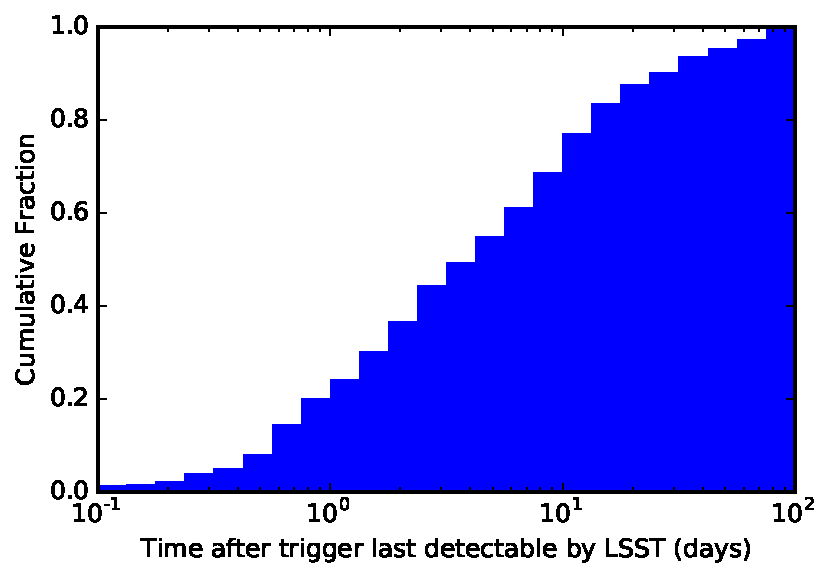
\includegraphics[width=0.6\textwidth]{figs/transients/afterglow_cdf.pdf}
}
\caption{ Cumulative fraction of GRB on-axis afterglows fainter than
magnitude 24.7 at a given time after the burst. We use an $\alpha=1$
decay with no jet breaks and the brightness parameters of
\citet{2011PASP..123.1034J}. }
\label{fig:afterglow_visibility}
\end{figure}

Thanks to LSST's depth, GRBs can be visible for weeks (Figure
\ref{fig:afterglow_visibility}).  Accordingly,
modest enhancements to the intra- and inter-night revisit rate with
single-filter rolling cadences should substantially improve LSST's
discovery and characterization of relativistic explosions.


\subsection{Conclusions}

Here we answer the ten questions posed in
\autoref{sec:intro:evaluation:caseConclusions}:

\begin{description}

\item[Q1:] {\it Does the science case place any constraints on the
tradeoff between the sky coverage and coadded depth? For example, should
the sky coverage be maximized (to $\sim$30,000 deg$^2$, as e.g., in
Pan-STARRS) or the number of detected galaxies (the current baseline
of 18,000 deg$^2$)?}

\item[A1:] No strong constraint, although on average
	larger sky coverage provides fewer epochs for the dense time sampling
	required to detect fast-fading events like GRBs.

\item[Q2:] {\it Does the science case place any constraints on the
tradeoff between uniformity of sampling and frequency of  sampling? For
example, a rolling cadence can provide enhanced sample rates over a part
of the survey or the entire survey for a designated time at the cost of
reduced sample rate the rest of the time (while maintaining the nominal
total visit counts).}

\item[A2:]  Frequency of sampling is far more important than uniformity of
	sampling for fast transients like GRBs.  Rolling cadences with
		three or more epochs per night or two are needed for
		realtime discovery of young events.

\item[Q3:] {\it Does the science case place any constraints on the
tradeoff between the single-visit depth and the number of visits
(especially in the $u$-band where longer exposures would minimize the
impact of the readout noise)?}

\item[A3:]  While greater single visit depth probes a greater cosmological
	volume within which to detect GRBs and other fast transients,
		our efficiency at discovering
		GRBs with LSST is driven entirely by the time sampling.
		Accordingly we prefer a larger number of visits per field
		to greater single-exposure depth, independent of band..

\item[Q4:] {\it Does the science case place any constraints on the
Galactic plane coverage (spatial coverage, temporal sampling, visits per
band)?}

\item[A4:] As GRBs are cosmological events, we expect to detect very few at
	low Galactic latitudes due to extinction.  Accordingly this
		science case is insensitive to observing plans in the Plane
		except insofar as they limit the number and cadence of
		exposures at higher latitudes.

\item[Q5:] {\it Does the science case place any constraints on the
fraction of observing time allocated to each band?}

\item[A5:] No strong constraints, although detection of faint afterglows
	will benefit from exposures taken in the bands with deepest
		single-exposure depth.

\item[Q6:] {\it Does the science case place any constraints on the
cadence for deep drilling fields?}

\item[A6:] Deep drilling fields provide an excellent opportunity to achieve
	the high time sampling required to discover GRBs while they are
		young.  As discussed above, a good fast transient cadence
		might have a \textit{minimum} of three visits
		in a night separated by an hour or two, preferably in a
		single filter, with revisits every night.

\item[Q7:] {\it Assuming two visits per night, would the science case
benefit if they are obtained in the same band or not?}

\item[A7:] Due to the need to constrain the lightcurve shape, it is best if
	the observations are in the same filter--especially with only two
	visits per night.  Otherwise there is a degeneracy between the
	(evolving) color of the event and its lightcurve shape.

\item[Q8:] {\it Will the case science benefit from a special cadence
prescription during commissioning or early in the survey, such as:
acquiring a full 10-year count of visits for a small area (either in all
the bands or in a  selected set); a greatly enhanced cadence for a small
area?}

\item[A8:] A dedicated experiment providing enhanced cadences over a small
	area  (as described above) would provide an ideal
	experiment to determine the rate of fast transients.  Such an
	observing strategy would also
	facilitate organizing necessary followup resources
	(spectroscopy, X-ray followup) because the observing period would
	be known in advance.

\item[Q9:] {\it Does the science case place any constraints on the
sampling of observing conditions (e.g., seeing, dark sky, airmass),
possibly as a function of band, etc.?}

\item[A9:] None unique to the science.

\item[Q10:] {\it Does the case have science drivers that would require
real-time exposure time optimization to obtain nearly constant
single-visit limiting depth?}

\item[A10:] No.

\end{description}

\navigationbar


% --------------------------------------------------------------------

% PJM: moved to Future Work while MAF analysis is pending:
% % ====================================================================
%+
% SECTION:
%    tde.tex
%
% CHAPTER:
%    transients.tex
%
% ELEVATOR PITCH:
%    Tidal disruption events (TDEs) are the disruptions of stars by supermassive black holes.
%    They can produce flares in the optical and UV (sometimes accompanied by X-ray and radio emission as well).
%    These flares can be used to reveal the properties of otherwise quiescent SMBHs and to study accretion physics.
%    TDEs are rare, LSST will allow the first statistical sample of such events.
%
% AUTHORS:
%    Iair Arcavi (@arcavi)
%
% ====================================================================

% \section{Tidal Disruption Events}
\subsection{Tidal Disruption Events}
\def\secname{\chpname:tdes}\label{sec:\secname}

\credit{arcavi}

A star passing close to a supermassive black hole (SMBH;
$M\gtrsim10^{6}M_{\odot}$) will be torn apart by tidal forces. For
certain ($\lesssim10^{8}M_{\odot}$) black hole masses, the disruption
will occur outside the event horizon and will be accompanied by an
observable flare \citep{Hills1975, Rees1988}. Such flares can be used to
study inactive SMBHs, which are otherwise inaccessible beyond the nearby
($\lesssim100$ Mpc) universe.

We are now building our understanding of how observational properties of
TDEs are affected by the SMBH. Theory claims to provide such a
connection \citep[e.g.][]{Lodato2009, Guillochon2014}, but uncertainties
in the physics of the disruption, subsequent accretion and emission
mechanisms are currently topics of debate \citep[e.g.][]{Strubbe2015,
Guillochon2014, Roth2015}, and new models are vigorously being developed
\citep[e.g.][]{Piran2015, Hayasaki2015, Svirski2015, Bonnerot2015}.

TDEs are rare ($\sim10^{-5}-10^{-4}$ events per galaxy per year;
\citealp{Wang2004, Stone2015}), and until recently, TDE candidates were
discovered mostly in archival data \citep[e.g.][]{Donley2002,
Gezari2006, Esquej2007}. Now, however, wide-field transient surveys have
started discovering TDEs in real time.

Generally, two types of TDE candidates have been identified:
\begin{enumerate}
	\item \textit{High energy TDEs}. The prototype is Swift J1644
\citep{Bloom2011, Burrows2011, Levan2011, Zauderer2011}, with two other
events known \citep{Cenko2012, Brown2015}. These events display emission
in $\gamma$-rays and X-rays as well as in the radio, but are not
detected in the optical.
\item \textit{Optical-UV TDEs}.  The prototype is PS1-10jh
(Figure \ref{fig:tde}; \citealp{Gezari2012}).
		About $8$ other events are known
\citep{Chornock2014, Arcavi2014, Holoien2014, Holoien2015, Holoien2016}.
Some events were detected also in the X-rays and radio (in addition to
the optical and UV), but the X-ray and radio signatures are different
than those of the high energy TDE candidates.
\end{enumerate}

\begin{figure}[hbt]
\centerline{
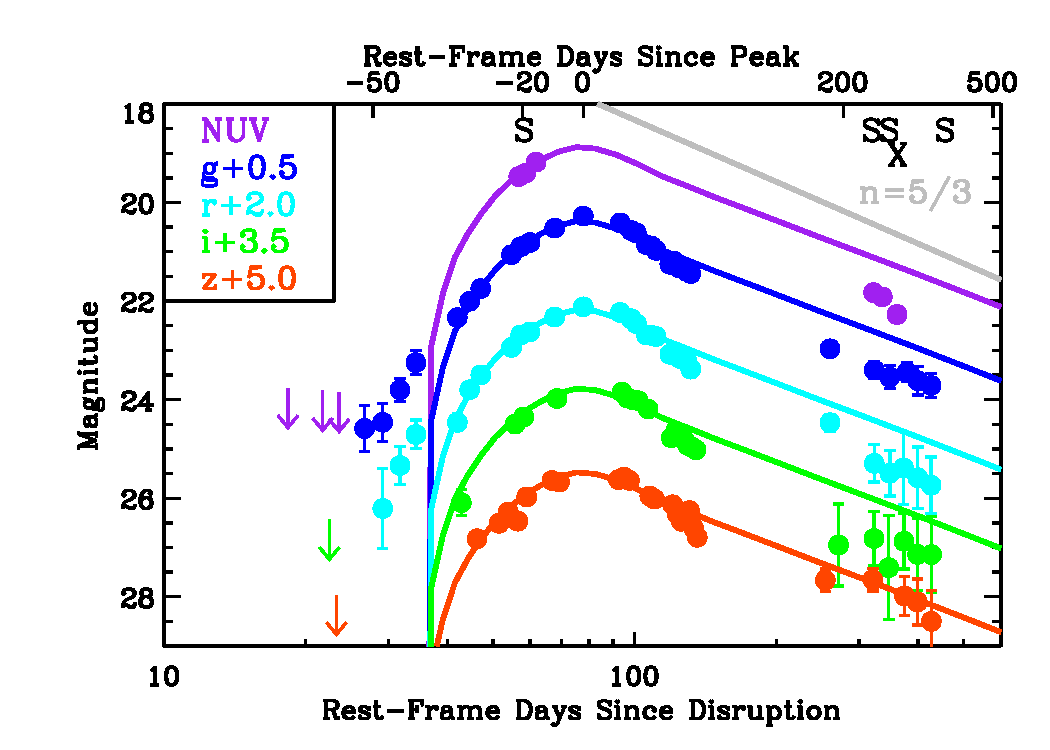
\includegraphics[width=0.6\textwidth]{figs/transients/tdeGezari.pdf}
}
\caption{
Optical and near-UV lightcurve of the TDE PS1-10jh \citep{Gezari2012}.
}
\label{fig:tde}
\end{figure}

It is still not clear whether both of these classes of transients are TDEs,
and if so, why they are so different form each other. One option raised is
that some TDEs may launch jets, which when directed towards us, appear as
the high energy events, but otherwise appear as the optical-UV events.
It is still not clear if this is indeed the case \citep[e.g.][]{VanVelzen2013}.

Here we focus on the second type of TDE candidates, which is the
relevant class for LSST, since they can be discovered in the optical.
However, multi-wavelength coordinated observations of
optically-discovered events are required in order to better understand
the connection between the two types of candidates.

The first well-sampled TDE of the optical+UV class was PS1-10jh (discovered by Pan-STARRS;
\citealt{Gezari2012}). \citet{Arcavi2014} later presented three new TDE candidates
from PTF and one discovered by ASAS-SN, all with similar properties
as PS1-10jh. These events exhibit blue colors, broad light curves,
peak absolute magnitudes of $\sim-20$ and a $\sim t^{-5/3}$ decay
at late times. This decay law has been suggested as a unique signature
of accretion-powered TDE light curves \citep{Rees1988, Evans1989, Phinney1989}.
Early-time deviations from the $t^{-5/3}$ rate
can be used to constrain the density profile of the disrupted star
\citep{Lodato2009, Gezari2012}. Late-time deviations would
test the accretion power-source hypothesis altogether.

The spectral signatures of these TDEs are still a puzzle. PS1-10jh displayed
only He II emission lines, lacking any signs of H. Some of the \citet{Arcavi2014}
sample, however, do display H emission.
In fact, a continuum of H / He emission ratios for this class of transients
is being revealed, and is now a focus of theoretical modelling \citep{Strubbe2015, Roth2015}.

The second recent discovery relating to this new sample concerns their
host galaxies \citep{Arcavi2014, French2016}, most of which are
post-starburst galaxies. These galaxies show little or no signs of on-going star formation, but their significant A stellar populations indicate that star formation ceased abruptly a few hundred Myr to a Gyr ago \citep{Dressler1983}. Galaxies with these characteristics often show signs of recent galaxy-galaxy mergers \citep{Zabludoff1996}, which produced the starburst and evolved the bulge. Optical-UV TDEs are intrinsically over abundant in post-starburst galaxies by a factor of $\sim30-200$ (depending on the characteristics of the galaxy; \citealt{French2016}). The reason for the strong preference of TDEs for post-starburst galaxies has still not been determined.

LSST's contribution to TDE studies will be substantial.
\citet{VanVelzen2011} estimate that LSST could discover approximately
4000 TDEs per year. The main drivers for studying TDEs with LSST are:
\begin{itemize}
\item Measuring black hole masses: This involves fitting models to TDE
light curves. It is also relevant to correlate these measurements with
host galaxy properties (mass, bulge/disk decomposition).
\item Constraining galactic dynamics by measuring the TDE rates as
functions of black hole mass and galaxy types.
\item Characterizing TDE emission signatures.
\end{itemize}

A metric is required for measuring how well TDEs can be identified and
distinguished from supernovae and active galactic nuclei. In general, we
expect TDEs to:
\begin{itemize}
\item Be located in the center of their host.
\item Display approximately constant blue (few $10^4$K) colors.
\item Evolve slowly (weeks-months).
\item Not show past AGN-like variability.
\item Preferentially peak around mag -20.
\item Preferentially be hosted in a post-starburst galaxy.
\end{itemize}
These criteria are based on our current knowledge of optical TDEs, which
is still in its early stages. The field is rapidly evolving, and it is
possible that new observations will change the current picture of TDE
emission. This metric is probably best combined with those discussed in
 \autoref{sec:\chpname:SNtransients} for identifying supernovae, though the
luminosity function of TDEs (or what constitutes a ``typical'' TDE light
curve) is not yet known.

A second metric is required to asses the accuracy with which the black
hole mass can be constrained from the TDE light curves. This metric can
be based on existing theoretical models to fit simulated TDE light
curves (such as TDEFit; \citealt{Guillochon2014}).

% ====================================================================
%
 \subsection{Conclusions}

 Here we answer the ten questions posed in
 \autoref{sec:intro:evaluation:caseConclusions}:

 \begin{description}

 \item[Q1:] {\it Does the science case place any constraints on the
 tradeoff between the sky coverage and coadded depth? For example, should
 the sky coverage be maximized (to $\sim$30,000 deg$^2$, as e.g., in
 Pan-STARRS) or the number of detected galaxies (the current baseline
 of 18,000 deg$^2$)?}

 \item[A1:] The number of events discovered will be approximately proportional to the sky area surveyed, multiplied by the
 average length of coverage, so added sky area is beneficial, as long as the observing season per field is not shortened.

 \item[Q2:] {\it Does the science case place any constraints on the
 tradeoff between uniformity of sampling and frequency of  sampling? For
 example, a rolling cadence can provide enhanced sample rates over a part
 of the survey or the entire survey for a designated time at the cost of
 reduced sample rate the rest of the time (while maintaining the nominal
 total visit counts).}

 \item[A2:] Uniform sampling is optimum.

 \item[Q3:] {\it Does the science case place any constraints on the
 tradeoff between the single-visit depth and the number of visits
 (especially in the $u$-band where longer exposures would minimize the
 impact of the readout noise)?}

 \item[A3:] No, as long as all filters are well represented.

 \item[Q4:] {\it Does the science case place any constraints on the
 Galactic plane coverage (spatial coverage, temporal sampling, visits per
 band)?}

 \item[A4:] This science will be accomplished away from the galactic plane.

 \item[Q5:] {\it Does the science case place any constraints on the
 fraction of observing time allocated to each band?}

 \item[A5:] Increased $u$-filter cadence valuable for TDE.

 \item[Q6:] {\it Does the science case place any constraints on the
 cadence for deep drilling fields?}

 \item[A6:] Only cadences that sample timescales of weeks and greater will be useful.

 \item[Q7:] {\it Assuming two visits per night, would the science case
 benefit if they are obtained in the same band or not?}

 \item[A7:] Different bands would be strongly preferred.

 \item[Q8:] {\it Will the case science benefit from a special cadence
 prescription during commissioning or early in the survey, such as:
 acquiring a full 10-year count of visits for a small area (either in all
 the bands or in a  selected set); a greatly enhanced cadence for a small
 area?}

 \item[A8:] A sparse cadence applied to a large sky area would be scientifically productive, but this is not a strong constraint.

 \item[Q9:] {\it Does the science case place any constraints on the
 sampling of observing conditions (e.g., seeing, dark sky, airmass),
 possibly as a function of band, etc.?}

 \item[A9:] No.

 \item[Q10:] {\it Does the case have science drivers that would require
 real-time exposure time optimization to obtain nearly constant
 single-visit limiting depth?}

 \item[A10:] No.

 \end{description}

 \navigationbar


% --------------------------------------------------------------------

% PJM: moved to Future Work while MAF analysis is pending:
% % ====================================================================
%+
% SECTION:
%    cv.tex
%
% CHAPTER:
%    transients.tex
%
% ELEVATOR PITCH:
%    Explain in a few sentences what the relevant discovery or
%    measurement is going to be discussed, and what will be important
%    about it. This is for the browsing reader to get a quick feel
%    for what this section is about.
%
% AUTHORS:
%    Federica Bianco (@fedhere)
%
% ====================================================================

% \section{Cataclismic Variables}
\subsection{Cataclismic Variables}
\def\secname{\chpname:CVtransients}\label{sec:\secname}

\credit{paulaszkody},
\credit{fedhere}

Cataclysmic Variables (CVs) encompass a broad group of objects
including novae, dwarf novae, novalikes, and AM CVn systems, all with different
amplitudes and rate of variability. The one thing they all have in
common is active mass transfer from a late type companion to a
white dwarf. These create variability on a wide range of timescales:

\begin{itemize}
	\item \textit{minutes} flickering in
dwarf novae and novalikes, pulsations in accreting white dwarfs in
the instability strip, orbital periods of AM CVn systems
\item \textit{hours} orbital periods of novae, dwarf novae and novalikes
\item \textit{days} normal outburst lengths of dwarf novae
\item \textit{weeks} outburst length of superoutbursts in short orbital period
dwarf novae, outburst recurrence time of normal outbursts in short
orbital period dwarf novae
\item \textit{months} outburst recurrence time of
longer period dwarf novae, various state changes in novalikes, declines
in novae
\item \textit{years} for the outburst recurrence timescales of the
shortest period dwarf novae and the recurrence times in recurrent novae
\end{itemize}
The
amplitudes range from tenths of mags for flickering and pulsations to 4 mags
for normal dwarf novae and changes in novalike states up to 9-15 mags for the
largest amplitude dwarf novae and classical novae.

These large differences make correct classification with LSST difficult
but necessary in order to reach goals of assessing the correct number
of types of objects for population studies of the end points of
binary evolution. Multiple filters (especially the blue $u$ and $g$)
along with amplitude and recurrence of variation provide the best
discrimination, as all CVs are bluer during outburst and high states of
accretion. Long term, evenly sampled observations can provide indications
of the low amplitude random variability and catch some of the more frequent
outbursts, but higher sampling is needed to determine whether an object
has a normal or superoutburst, to catch a rise to outburst or to a
different accretion state or to follow a nova. Novae typically
have rise times of a few days, while the decline time and shape provide
information as to the mass, distance and composition. The time to decline
by 2-3 magnitudes is correlated with composition,
%
% FED: what is a range of time scales for this decline? days? months?
%
WD mass and location in
the galaxy, thus enabling a study of Galactic chemical evolution.  As with SN,
the diagnostic power for all these systems rests on color and sampling.

Metrics to be developed would assess the abilities of  a given observing
strategy to distinguish between new novae and dwarf novae outbursts and
identify high and low states.  This discriminiation is provided by
measurement of the shapes and recurrence times of large variations as well
as blue colors to distinguish low amplitude variability that would indicate
new pulsators or novalikes. Population studies rely on the numbers of long
orbital period (low amplitude, wide outbursts) vs. short orbital period
(patterns of short outbursts followed by larger, longer superoutbursts)
dwarf novae at different places in the galaxy, as well as the numbers of
recurrent (1-10 yrs) vs. normal novae (10,000 yrs, about 35/galaxy/yr).
Objects particulary worthy of later followup are containing highly magnetic
white dwarfs. These objects can be identified in a large sample when the
magnitude for a majority of the years is a faint (low) state and a small
percentage of time is a bright (high) state, combined with a red color (due
to cyclotron emission from the magnetic accretion column).

% ====================================================================
%
\subsection{Conclusions}
%
% Here we answer the ten questions posed in
% \autoref{sec:intro:evaluation:caseConclusions}:
%
 \begin{description}

 \item[Q1:] {\it Does the science case place any constraints on the
 tradeoff between the sky coverage and coadded depth? For example, should
 the sky coverage be maximized (to $\sim$30,000 deg$^2$, as e.g., in
 Pan-STARRS) or the number of detected galaxies (the current baseline
 of 18,000 deg$^2$)?}

 \item[A1:] Extending the sky area is not a priority for this science.

 \item[Q2:] {\it Does the science case place any constraints on the
 tradeoff between uniformity of sampling and frequency of  sampling? For
 example, a rolling cadence can provide enhanced sample rates over a part
 of the survey or the entire survey for a designated time at the cost of
 reduced sample rate the rest of the time (while maintaining the nominal
 total visit counts).}

 \item[A2:] Intervals of higher cadence are extremely valuable and a rolling cadence is a
satisfactory approach, subject to cadence details.

 \item[Q3:] {\it Does the science case place any constraints on the
 tradeoff between the single-visit depth and the number of visits
 (especially in the $u$-band where longer exposures would minimize the
 impact of the readout noise)?}

 \item[A3:] Increasing the number of $u$-band visits will improve the characterization of CV phenomena.

 \item[Q4:] {\it Does the science case place any constraints on the
 Galactic plane coverage (spatial coverage, temporal sampling, visits per
 band)?}

 \item[A4:] Most CVs will be detected in the galactic plane, and a long, rich series of visits is needed.

 \item[Q5:] {\it Does the science case place any constraints on the
 fraction of observing time allocated to each band?}

 \item[A5:] $u$-band is diagnostic, especially $u$-$g$.

 \item[Q6:] {\it Does the science case place any constraints on the
 cadence for deep drilling fields?}

 \item[A6:] For deep drilling in the galactic plane or for local group galaxies, the best cadences would obtain several epochs  per night in
 each filter, rather than concentrating all acquisition with a filter in a single rapid burst.

 \item[Q7:] {\it Assuming two visits per night, would the science case
 benefit if they are obtained in the same band or not?}

 \item[A7:] Same filter and different filter each offer valuable information, and a mix of these two options would be preferred
pending test of both cadences.

 \item[Q8:] {\it Will the case science benefit from a special cadence
 prescription during commissioning or early in the survey, such as:
 acquiring a full 10-year count of visits for a small area (either in all
 the bands or in a  selected set); a greatly enhanced cadence for a small
 area?}

 \item[A8:] It would be very helpful to CV studies - and many other areas of transient science - to understand variability across all timescales.
 Especially valuable would be a cadence that would cover one (cluster, rich star field) with all the timescales that will not be
strongly represented  in the main survey, starting at 15 seconds.

 \item[Q9:] {\it Does the science case place any constraints on the
 sampling of observing conditions (e.g., seeing, dark sky, airmass),
 possibly as a function of band, etc.?}

 \item[A9:] No.

 \item[Q10:] {\it Does the case have science drivers that would require
 real-time exposure time optimization to obtain nearly constant
 single-visit limiting depth?}

 \item[A10:] No.

 \end{description}

 \navigationbar


% --------------------------------------------------------------------

% PJM: moved to Future Work while MAF analysis is pending:
% % ====================================================================
%+
% SECTION:
%    eruptive.tex
%
% CHAPTER:
%    transients.tex
%
% ELEVATOR PITCH:
%-
% ====================================================================

% \section{LBVs and related non-supernova transients}
\subsection{LBVs and related non-supernova transients}
\def\secname{\chpname:LBVs}\label{sec:\secname}

\credit{nathansmith}

There is a large and diverse class of visible-wavelength transient
sources recognized in nearby galaxies that appear to be distinct from
traditional novae and from SNe, and have often been associated with
the giant eruptions of luminous blue varibles (LBV), such as the 19th
century outburst of $\eta$ Carinae.  Broadly speaking, members of this
class of transients share the common properties that they have peak
luminosities below those of most core-collapse SNe and more luminous
than novae and CVs (absolute magnitudes of roughly $-$9 to $-$15 mag).
They also have H-rich spectra (usually) with relatively narrow lines
that indicate modest bulk outflow velocities of 10$^2$ to 10$^3$ km
s$^{-1}$ (although some have exhibited small amounts of material at
faster speeds).  They tend to evolve on fairly long timescales of
weeks to years (although sometimes they exhibit a quick rise to peak
similar to SNe II-P). This group of transients has gone by many names,
such as LBV eruptions, SN impostors, Type V supernovae,
intermediate-luminosity optical (or red) transients, as well as others
that often include a physical interpretation.
%For brevity, these are
%often collectively referred to as ``LBVs'', although many of them may
%not actually be LBVs.
%This may be largely for historical reasons,
%since LBVs were the first of these to be recognized as a class.  Some
%of the subgroups may be very different from objects like $\eta$
%Carinae, however.

Observationally, these eruptions are understood to represent important
and dramatic mass-loss episodes in the lives of massive stars, based
on empirical estimates of the amount of ejected matter.
%Guided
%largely by nearby LBVs with resolved shells, t
These eruptions are
expected to instigate mass loss that is comparable to or more
important than metallicity-dependent winds of massive stars.  This
mode of mass loss, regardless of the mechanism, may be a very
important ingredient in the evolution of massive stars that is
currently not included in stellar evolution models.  Correcting this
is one of the key science drivers in trying to understand the physics
these eruptions.

%The degeneracy
%arises because when the objects are
%fully obscured by dust, one cannot actually meaure the star's
%temperature, and the bolometric luminosities of super-AGB and red and
%blue supergiants overlap.  Unfortunately,
%cases when we have strong constraints on the quiescent progenitor are
%rare, and once they reach their peak luminosity, there is a great deal
%of overlap in observed properties.

Theoretically, these eruptions are not understood.  %There are many
%ideas, but few if any confirmed mechanisms tied to observed
%objects.
Some
%previously discussed
theoretical ideas involve (1)
winds driven by super-Eddington instabilities (although the root cause
for suddenly exceeding the Eddington limit remains unexplained), (2)
hydrodynamic explosions caused by deep-seated energy deposition, such
as unsteady nuclear burning, (3) accretion onto companion stars in
binary systems (degenerate or not), (4) mergers in binary and triple
systems, (5) electron-capture SNe, and (6) ``failed SNe'' associated
with a weak explosion and envelope ejection that results from black
hole formation during core collapse.
Because of the relatively low total energy indicated by
radiative luminosities and outflow speeds, these are usually discussed
as non-terminal eruptions, however, the last two are terminal events
that are less luminous and lower energy than normal SNe, and the last
3 should only occur once for a given source.
%Together with several well-studied examples that indicate
%repeating eruptions, there are indeed many
%cases where only one such transient has been seen at the same
%position, and some cases where late-time observations suggest that no
%source has survived with a luminosity comparable to its progenitor.
%However, there are also several well-studied examples that indicate
%repeating eruptions (multiple repeating transients, multiple nebular
%shells with different ages, etc).
All these theoretical mechanisms
may lead to similar observed phenomena: weak explosions, moderate
luminosities, slow expansion, dusty aftermath, but this class of objects
may represent a mixed-bag of different mechanisms that get lumped
together by default as ``other'' because they are not traditional SNe.

Rates for these LBV-like eruptions are still very poorly constrained;
%largely because most previous SN and transient searches with small
%telescopes have been optimized for finding more luminous SNe in a
%larger volume.  This field begun to change with recent surveys, and will
%be revolutionized with LSST.  F
%from discovered examples we have,
numbers are very roughly consistent with a volumetric rate comparable
to that of core-collapse SNe or larger.  %, but with a large error bar.
Limited information often makes classification into various
subgroups difficult or highly subjective, thus subclass rates are even
less well constrained.  %The ``rate'' also depends on how
%faint the lower limit of inclusions is; e
Evidence suggests that the brightest events occurr less frequently and that
numbers increase as one moves to lower luminosity.  At the faint end,
it becomes difficult to distinguish between eruptions and regular
variability of LBVs, or between massive star eruptions and CVs.  \emph{With
deep LSST stacks identifying faint CV in quiescent states this will
 change dramatically in the LSST age, with the unvailing of
detailed progenitor information}.  Having deep, pre-eruption
characterization of sources at the positions of these eruptive
transients (as well as SN precursors) will likely be a major
contribution of LSST.
An important empirical discriminant of subgroups in this class comes
from their progenitor stars.  Some are indeed seen to be very
luminous, blue supergiant stars consistent with traditional LBVs.
Some, however, have somewhat less luminous, heavily dust-obscured
progenitor stars that have been associated with either dust-enshrouded
blue or red supergiants, or alternatively, with super-AGB stars of
8-10 M$_{\odot}$%, with uncertainty.


An area of recent interest is that eruptive non-terminal transients
have been observed, in some cases, to precede much more powerful
explosions that are seen as Type IIn supernovae.  \emph{Detectability of SN
precursors eruptions is discussed in ~\autoref{chp:galaxy}.
LSST can provide a large enough sample of these events to enable the study
or rates.} %There may also be
SN
precursors have observed or inferred properties that are very similar
to LBVs and related transients,
%.  This may suggest some link between them,
but then again, most of the LBVs and other SN impostors have been
observed for decades and have not gone SN (yet).  \emph{Being able to
  distinguish which of these optical transients are SN precursors and
  which are not is a major science driver.}  The amount of mass lost
in a precursor eruption may dramatically alter the type of SN that is
observed.  Even if the pre-SN transients are not observed directly,
pre-SN eruptive mass loss can be inferred and constrained with
persistent observations of the detected eruptions' lightcurves (and
spectra) through circumstellar interaction diagnostocs of
the bright eruptions and explosions.
%a continuum of energies in pre-SN outbursts, extending down to more
%normal classes of core-collapse SNe, but these may often go
%unrecognized unless the SN is caught very early after explosion.

In terms of timescales, many of the eruptive transients exhibit rise
and decline timescales similar to normal SNe~II-P or II-L, but with
fainter peak luminosity.  For these, observational cadence
requirements will be the same as SNe.  For some eruptive transients,
however, the rise timescales can be very long (rising a few magnitudes
in years).  While LSST's cadence will certainly be fast enough, being
able to discover slowly rising transients that do not change much from
night to night will be an important metric, and the edge effects
should be investigated.
For the faster-rising transients, just like for SNe, spectroscopic
follow-up is needed to discriminate these from normal SNe, and also
contextual information about the host galaxy (and hence, the absolute
magnitude) is needed to differentiate these non-terminal eruptions
from Type IIn supernovae (their spectra look similar, although LBVs do
tend to have narrower lines).  %Spectral and color evolution, as well
%as information about the progenitor, is needed to distinguish among
%subgroups within the class.
Multiwavelength follow-up is often extremely valuable or even
essential; i.e. mid-IR tells us if an optically invisible source is
cloaked in a dust shell but still quite luminous; Xrays and radio tell
us if an expanding shock wave is the likely source of persistent
luminosity.  For these reasons, nearby cases will continue to be the
most valuable in deciphering the physics of subclasses, whereas the
increased volume in which LSST discovers these fainter transients will
drastically improve our understanding of their rates.  Armed with both
a better understanding of their underlying physics and
characterization, as well as their rates and duty cycles, these
eruptive events can then be incorporated into stellar evolution models
and population synthesis/feedback models.

% % --------------------------------------------------------------------
%
% \subsection{Metrics}
% \label{sec:\secname:metrics}
%
% % --------------------------------------------------------------------
%
% \subsection{OpSim Analysis}
% \label{sec:\secname:analysis}
%
% % --------------------------------------------------------------------
%
% \subsection{Discussion}
% \label{sec:\secname:discussion}
%
% ====================================================================
%
% \subsection{Conclusions}
%
% Here we answer the ten questions posed in
% \autoref{sec:intro:evaluation:caseConclusions}:
%
% \begin{description}
%
% \item[Q1:] {\it Does the science case place any constraints on the
% tradeoff between the sky coverage and coadded depth? For example, should
% the sky coverage be maximized (to $\sim$30,000 deg$^2$, as e.g., in
% Pan-STARRS) or the number of detected galaxies (the current baseline
% of 18,000 deg$^2$)?}
%
% \item[A1:] ...
%
% \item[Q2:] {\it Does the science case place any constraints on the
% tradeoff between uniformity of sampling and frequency of  sampling? For
% example, a rolling cadence can provide enhanced sample rates over a part
% of the survey or the entire survey for a designated time at the cost of
% reduced sample rate the rest of the time (while maintaining the nominal
% total visit counts).}
%
% \item[A2:] ...
%
% \item[Q3:] {\it Does the science case place any constraints on the
% tradeoff between the single-visit depth and the number of visits
% (especially in the $u$-band where longer exposures would minimize the
% impact of the readout noise)?}
%
% \item[A3:] ...
%
% \item[Q4:] {\it Does the science case place any constraints on the
% Galactic plane coverage (spatial coverage, temporal sampling, visits per
% band)?}
%
% \item[A4:] ...
%
% \item[Q5:] {\it Does the science case place any constraints on the
% fraction of observing time allocated to each band?}
%
% \item[A5:] ...
%
% \item[Q6:] {\it Does the science case place any constraints on the
% cadence for deep drilling fields?}
%
% \item[A6:] ...
%
% \item[Q7:] {\it Assuming two visits per night, would the science case
% benefit if they are obtained in the same band or not?}
%
% \item[A7:] ...
%
% \item[Q8:] {\it Will the case science benefit from a special cadence
% prescription during commissioning or early in the survey, such as:
% acquiring a full 10-year count of visits for a small area (either in all
% the bands or in a  selected set); a greatly enhanced cadence for a small
% area?}
%
% \item[A8:] ...
%
% \item[Q9:] {\it Does the science case place any constraints on the
% sampling of observing conditions (e.g., seeing, dark sky, airmass),
% possibly as a function of band, etc.?}
%
% \item[A9:] ...
%
% \item[Q10:] {\it Does the case have science drivers that would require
% real-time exposure time optimization to obtain nearly constant
% single-visit limiting depth?}
%
% \item[A10:] ...
%
% \end{description}
%
% ====================================================================
%
\navigationbar


% --------------------------------------------------------------------

% ====================================================================
%+
% SECTION:
%    gw.tex
%
% CHAPTER:
%    transients.tex
%
% ELEVATOR PITCH:
%-
% ====================================================================

\section{Gravitational Wave Sources}
\def\secname{\chpname:gw}\label{sec:\secname}

\credit{raffaellamargutti},
\credit{Doctor},
\credit{Fong},
\credit{Haiman},
\credit{Kalogera},
\credit{Trimble},
\credit{Zauderer}

The first detection of Gravitational Waves (GW) by the advanced
LIGO/Virgo collaboration \citep{Abbott16, Abbott09, Acernese08} has
recently opened a new window of exploration into our Universe. The
amount of information that can be revealed by the properties of the GW
emission is immense and holds promises for revolutionary insights,
including accurate masses and spins of neutron stars and black holes,
tests of General Relativity and an accurate census of the neutron star
(NS) and black hole (BH) populations that might challenge our current
understanding of massive stellar evolution. However, GW events are
poorly localized (10-100 deg$^2$ at the time of LSST operations). The
identification of EM counterparts would provide precise localization and
distance measurements, in addition to the necessary astrophysical
context (e.g. host galaxy properties, connection to specific stellar
populations) to fully exploit the revolutionary power of this new GW
era.

% --------------------------------------------------------------------

\subsection{Target measurements and discoveries}
\label{sec:\secname:targets}

The first GW event was found to be associated with the merger of two
black holes \citep{Abbott16,Abbott16b}. Although no EM counterpart was
expected to accompany a black-hole black-hole (BBH) merger, it seems now
possible that even BBH mergers  might produce short GRB-like EM emission
\citep{Connaughton16,Loeb16,Zhang16,Perna16,Stone16}. Indeed, in
analogy with supermassive BH mergers, shocks might develop in the
just-formed circumbinary accretion disk (if a disk forms), which can
produce a bright afterglow following the BBH merger (e.g.
\citealt{Lippai08,Corrales10,Schnittman13}). Albeit speculative in
nature, it is advisable to keep an open mind about the possibility of EM
counterparts to BBH mergers.

The most promising and better understood EM counterparts to GW events
are ``kilonovae" \citep{Li98,Metzger10,Metzger12,Kasen13,Barnes13}.
Kilonovae are short-lived (typical time scale of one week), apparently
faint ($z\sim21$ mag at peak at 120 Mpc), red ($i-z\approx1$ mag),
isotropic transients (\autoref{Fig:kilonova}) due to the radioactive
decay of r-process elements synthesized in the merger ejecta of a NS-NS
or NS-BH system. These merging systems are the favored progenitors of
short GRBs. Indeed, a signature consistent with kilonova emission has been
recently found following the short GRB\,130603B
\citep{Berger13,Tanvir13}. The key piece of information that enabled the
discovery of kilonova-like emission associated with  this short GRB was
its sub-arcsecond localization enabled by the detection of the optical
afterglow, which allowed for an effective kilonova search with the
Hubble Space Telescope (\autoref{Fig:kilonova}). In contrast, the
typical localization region of GW events in the LSST era is expected to
be of the order of a few tens of square degrees \citep{aaa+13}. It is
thus clear that the major challenges faced by the optical follow-up of
GW events is represented by the combination of poor localizations with
faint and fast evolving red electromagnetic counterparts.

The detection of an optical counterpart in conjunction with a GW event
will significantly leverage the GW signal. LSST, with its the wide FOV,
wavelength coverage and exquisite sensitivity is uniquely poised to
identify and characterize counterparts to GW events.

\begin{figure}
\vskip -0.0 true cm
\centering
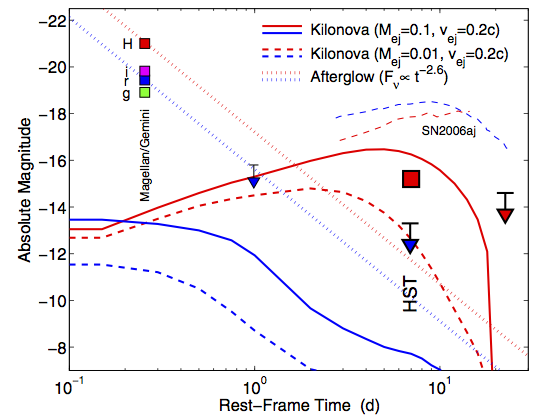
\includegraphics[scale=0.85]{figs/transients/kilonovaBerger.png}
\caption{Kilonova signature in the short GRB\,130603B as revealed by the
Hubble Space Telescope (HST). The Magellan and Gemini telescopes sampled
the optical afterglow of the GRB (dotted lines). The kilonova light
starts to dominate the emission in the H band around a few days after
the merger. Thick and dashed lines: theoretical kilonova models from
\citet{Barnes13} showing that kilonovae are fast-evolving, faint and red
transients. The light-curve of the SN\,2006aj associated with the long
GRB\,060218  is also shown for comparison. From \citet{Berger13}.}
\label{Fig:kilonova}
\end{figure}


% --------------------------------------------------------------------

\subsection{OpSim Analysis and Discussion}
\label{sec:\secname:analysis}

Effective follow up of GW triggers relies on the capability to sample a
relatively large portion of the sky, repeatedly, over a time scale $<1$
week, with different filters \citep{Cowperthwaite15}. In the optical
band, the kilonova signature is expected to be more prominent in the
$i$, $z$  and $y$ filters, which we identify as the most promising
filters for the kilonova search. We emphasize however that another set
of contemporaneous observations in  a ``bluer" filter is necessary to
acquire color information and distinguish kilonovae from other
fast-evolving transients.

We use the median inter-night gap  for visits in the same filter derived
from the candidate Baseline Cadence \opsimdbref{db:baseCadence} to show that,
in the absence of a Target of Opportunity (ToO) capability, it is
\emph{not} possible for LSST  to play a major role in the identification
of EM counterparts of GW triggers.

To identify kilonova candidates we need at least 2 observations acquired
within $\sim 1$ week  of the GW event \citep{Cowperthwaite15}. Using the
inter-night gap distribution for visits in the $y$ filter (which is the
most promising filter for a kilonova search), the area of the sky
covered with cadence  $\Delta t<7$ days at any given time, is
$A_{sky}\sim 3000$ deg$^2$ (including deep drilling fields).  This is
the area that can be searched for fast evolving transients.  Two
important considerations follow:

\begin{itemize}
\item[(1)] $A_{sky}$ only covers $P\sim7$\% of the sky. The  probability
that the \emph{entire} GW localization region is contained, by chance,
within $A_{sky}$ is thus very small.
\item[(2)] Even if LSST is able to cover a meaningful portion of the GW
region, we would still not have color information, and we would thus be
unable to filter out contaminating transients.
\end{itemize}

\textit{We conclude that relying on the serendipitous alignment of the
LSST fields with the GW localization map is not an effective strategy to
follow up GW triggers and identify their EM counterparts. We thus
strongly recommend a ToO capability as part of the baseline LSST
operations strategy.}

Ideally, the ToO capability will allow for imaging of the GW
localization map at least twice over $\Delta t\lesssim$1 week with a
``red" filter ($i$, $z$  or $y$),  and  will include the possibility to
designate a desired set of filters to obtain color information. By the
time of LSST operation the typical size of the GW localization region is
expected to be 10-100 deg$^2$, which would require a small number of
LSST re-pointings. We thus do \emph{not} anticipate a significantly
disruptive impact on other LSST campaigns (especially if only the GW
triggers with the best localizations in the southern sky are selected
for LSST ToOs).

\textit{At the price of re-shuffling a reasonably small number of
fields, \textbf{if} equipped with ToO capabilities, LSST can be the
premier player in the era of EM follow up to GW sources.}

% ====================================================================
%
% \subsection{Conclusions}
%
% Here we answer the ten questions posed in
% \autoref{sec:intro:evaluation:caseConclusions}:
%
% \begin{description}
%
% \item[Q1:] {\it Does the science case place any constraints on the
% tradeoff between the sky coverage and coadded depth? For example, should
% the sky coverage be maximized (to $\sim$30,000 deg$^2$, as e.g., in
% Pan-STARRS) or the number of detected galaxies (the current baseline 
% of 18,000 deg$^2$)?}
%
% \item[A1:] ...
%
% \item[Q2:] {\it Does the science case place any constraints on the
% tradeoff between uniformity of sampling and frequency of  sampling? For
% example, a rolling cadence can provide enhanced sample rates over a part
% of the survey or the entire survey for a designated time at the cost of
% reduced sample rate the rest of the time (while maintaining the nominal
% total visit counts).}
%
% \item[A2:] ...
%
% \item[Q3:] {\it Does the science case place any constraints on the
% tradeoff between the single-visit depth and the number of visits
% (especially in the $u$-band where longer exposures would minimize the
% impact of the readout noise)?}
%
% \item[A3:] ...
%
% \item[Q4:] {\it Does the science case place any constraints on the
% Galactic plane coverage (spatial coverage, temporal sampling, visits per
% band)?}
%
% \item[A4:] ...
%
% \item[Q5:] {\it Does the science case place any constraints on the
% fraction of observing time allocated to each band?}
%
% \item[A5:] ...
%
% \item[Q6:] {\it Does the science case place any constraints on the
% cadence for deep drilling fields?}
%
% \item[A6:] ...
%
% \item[Q7:] {\it Assuming two visits per night, would the science case
% benefit if they are obtained in the same band or not?}
%
% \item[A7:] ...
%
% \item[Q8:] {\it Will the case science benefit from a special cadence
% prescription during commissioning or early in the survey, such as:
% acquiring a full 10-year count of visits for a small area (either in all
% the bands or in a  selected set); a greatly enhanced cadence for a small
% area?}
%
% \item[A8:] ...
%
% \item[Q9:] {\it Does the science case place any constraints on the
% sampling of observing conditions (e.g., seeing, dark sky, airmass),
% possibly as a function of band, etc.?}
%
% \item[A9:] ...
%
% \item[Q10:] {\it Does the case have science drivers that would require
% real-time exposure time optimization to obtain nearly constant
% single-visit limiting depth?}
%
% \item[A10:] ...
%
% \end{description}

% ====================================================================

\navigationbar


% --------------------------------------------------------------------

% ====================================================================
%+
% SECTION:
%    transientFuture.tex
%
% CHAPTER:
%    transients.tex
%
% ELEVATOR PITCH:
%    Ideas for future metric investigation, with quantitaive analysis
%    still pending.
%-
% ====================================================================

\section{Future Work}
\def\secname{\chpname:future}\label{sec:\secname}

In this section we provide a short compendium of science cases that
are either still being developed, or that are deserving of quantitative
MAF analysis at some point in the future.

% ====================================================================

% ====================================================================
%+
% SECTION:
%    tde.tex
%
% CHAPTER:
%    transients.tex
%
% ELEVATOR PITCH:
%    Tidal disruption events (TDEs) are the disruptions of stars by supermassive black holes.
%    They can produce flares in the optical and UV (sometimes accompanied by X-ray and radio emission as well).
%    These flares can be used to reveal the properties of otherwise quiescent SMBHs and to study accretion physics.
%    TDEs are rare, LSST will allow the first statistical sample of such events.
%
% AUTHORS:
%    Iair Arcavi (@arcavi)
%
% ====================================================================

% \section{Tidal Disruption Events}
\subsection{Tidal Disruption Events}
\def\secname{\chpname:tdes}\label{sec:\secname}

\credit{arcavi}

A star passing close to a supermassive black hole (SMBH;
$M\gtrsim10^{6}M_{\odot}$) will be torn apart by tidal forces. For
certain ($\lesssim10^{8}M_{\odot}$) black hole masses, the disruption
will occur outside the event horizon and will be accompanied by an
observable flare \citep{Hills1975, Rees1988}. Such flares can be used to
study inactive SMBHs, which are otherwise inaccessible beyond the nearby
($\lesssim100$ Mpc) universe.

We are now building our understanding of how observational properties of
TDEs are affected by the SMBH. Theory claims to provide such a
connection \citep[e.g.][]{Lodato2009, Guillochon2014}, but uncertainties
in the physics of the disruption, subsequent accretion and emission
mechanisms are currently topics of debate \citep[e.g.][]{Strubbe2015,
Guillochon2014, Roth2015}, and new models are vigorously being developed
\citep[e.g.][]{Piran2015, Hayasaki2015, Svirski2015, Bonnerot2015}.

TDEs are rare ($\sim10^{-5}-10^{-4}$ events per galaxy per year;
\citealp{Wang2004, Stone2015}), and until recently, TDE candidates were
discovered mostly in archival data \citep[e.g.][]{Donley2002,
Gezari2006, Esquej2007}. Now, however, wide-field transient surveys have
started discovering TDEs in real time.

Generally, two types of TDE candidates have been identified:
\begin{enumerate}
	\item \textit{High energy TDEs}. The prototype is Swift J1644
\citep{Bloom2011, Burrows2011, Levan2011, Zauderer2011}, with two other
events known \citep{Cenko2012, Brown2015}. These events display emission
in $\gamma$-rays and X-rays as well as in the radio, but are not
detected in the optical.
\item \textit{Optical-UV TDEs}.  The prototype is PS1-10jh
(Figure \ref{fig:tde}; \citealp{Gezari2012}).
		About $8$ other events are known
\citep{Chornock2014, Arcavi2014, Holoien2014, Holoien2015, Holoien2016}.
Some events were detected also in the X-rays and radio (in addition to
the optical and UV), but the X-ray and radio signatures are different
than those of the high energy TDE candidates.
\end{enumerate}

\begin{figure}[hbt]
\centerline{
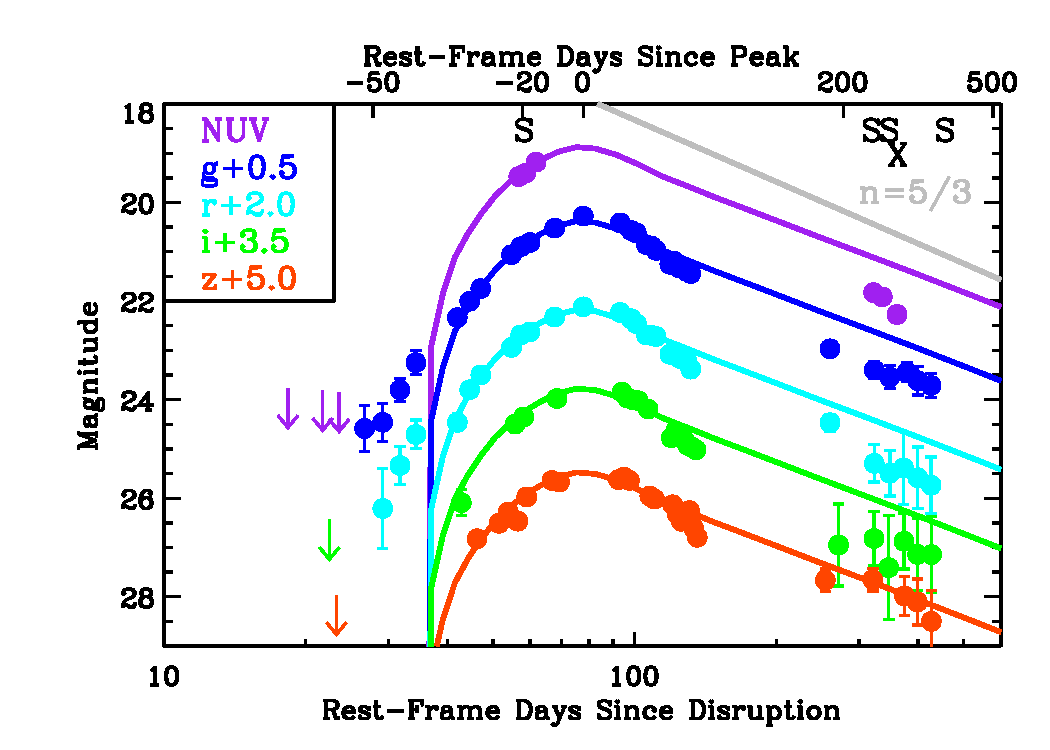
\includegraphics[width=0.6\textwidth]{figs/transients/tdeGezari.pdf}
}
\caption{
Optical and near-UV lightcurve of the TDE PS1-10jh \citep{Gezari2012}.
}
\label{fig:tde}
\end{figure}

It is still not clear whether both of these classes of transients are TDEs,
and if so, why they are so different form each other. One option raised is
that some TDEs may launch jets, which when directed towards us, appear as
the high energy events, but otherwise appear as the optical-UV events.
It is still not clear if this is indeed the case \citep[e.g.][]{VanVelzen2013}.

Here we focus on the second type of TDE candidates, which is the
relevant class for LSST, since they can be discovered in the optical.
However, multi-wavelength coordinated observations of
optically-discovered events are required in order to better understand
the connection between the two types of candidates.

The first well-sampled TDE of the optical+UV class was PS1-10jh (discovered by Pan-STARRS;
\citealt{Gezari2012}). \citet{Arcavi2014} later presented three new TDE candidates
from PTF and one discovered by ASAS-SN, all with similar properties
as PS1-10jh. These events exhibit blue colors, broad light curves,
peak absolute magnitudes of $\sim-20$ and a $\sim t^{-5/3}$ decay
at late times. This decay law has been suggested as a unique signature
of accretion-powered TDE light curves \citep{Rees1988, Evans1989, Phinney1989}.
Early-time deviations from the $t^{-5/3}$ rate
can be used to constrain the density profile of the disrupted star
\citep{Lodato2009, Gezari2012}. Late-time deviations would
test the accretion power-source hypothesis altogether.

The spectral signatures of these TDEs are still a puzzle. PS1-10jh displayed
only He II emission lines, lacking any signs of H. Some of the \citet{Arcavi2014}
sample, however, do display H emission.
In fact, a continuum of H / He emission ratios for this class of transients
is being revealed, and is now a focus of theoretical modelling \citep{Strubbe2015, Roth2015}.

The second recent discovery relating to this new sample concerns their
host galaxies \citep{Arcavi2014, French2016}, most of which are
post-starburst galaxies. These galaxies show little or no signs of on-going star formation, but their significant A stellar populations indicate that star formation ceased abruptly a few hundred Myr to a Gyr ago \citep{Dressler1983}. Galaxies with these characteristics often show signs of recent galaxy-galaxy mergers \citep{Zabludoff1996}, which produced the starburst and evolved the bulge. Optical-UV TDEs are intrinsically over abundant in post-starburst galaxies by a factor of $\sim30-200$ (depending on the characteristics of the galaxy; \citealt{French2016}). The reason for the strong preference of TDEs for post-starburst galaxies has still not been determined.

LSST's contribution to TDE studies will be substantial.
\citet{VanVelzen2011} estimate that LSST could discover approximately
4000 TDEs per year. The main drivers for studying TDEs with LSST are:
\begin{itemize}
\item Measuring black hole masses: This involves fitting models to TDE
light curves. It is also relevant to correlate these measurements with
host galaxy properties (mass, bulge/disk decomposition).
\item Constraining galactic dynamics by measuring the TDE rates as
functions of black hole mass and galaxy types.
\item Characterizing TDE emission signatures.
\end{itemize}

A metric is required for measuring how well TDEs can be identified and
distinguished from supernovae and active galactic nuclei. In general, we
expect TDEs to:
\begin{itemize}
\item Be located in the center of their host.
\item Display approximately constant blue (few $10^4$K) colors.
\item Evolve slowly (weeks-months).
\item Not show past AGN-like variability.
\item Preferentially peak around mag -20.
\item Preferentially be hosted in a post-starburst galaxy.
\end{itemize}
These criteria are based on our current knowledge of optical TDEs, which
is still in its early stages. The field is rapidly evolving, and it is
possible that new observations will change the current picture of TDE
emission. This metric is probably best combined with those discussed in
 \autoref{sec:\chpname:SNtransients} for identifying supernovae, though the
luminosity function of TDEs (or what constitutes a ``typical'' TDE light
curve) is not yet known.

A second metric is required to asses the accuracy with which the black
hole mass can be constrained from the TDE light curves. This metric can
be based on existing theoretical models to fit simulated TDE light
curves (such as TDEFit; \citealt{Guillochon2014}).

% ====================================================================
%
 \subsection{Conclusions}

 Here we answer the ten questions posed in
 \autoref{sec:intro:evaluation:caseConclusions}:

 \begin{description}

 \item[Q1:] {\it Does the science case place any constraints on the
 tradeoff between the sky coverage and coadded depth? For example, should
 the sky coverage be maximized (to $\sim$30,000 deg$^2$, as e.g., in
 Pan-STARRS) or the number of detected galaxies (the current baseline
 of 18,000 deg$^2$)?}

 \item[A1:] The number of events discovered will be approximately proportional to the sky area surveyed, multiplied by the
 average length of coverage, so added sky area is beneficial, as long as the observing season per field is not shortened.

 \item[Q2:] {\it Does the science case place any constraints on the
 tradeoff between uniformity of sampling and frequency of  sampling? For
 example, a rolling cadence can provide enhanced sample rates over a part
 of the survey or the entire survey for a designated time at the cost of
 reduced sample rate the rest of the time (while maintaining the nominal
 total visit counts).}

 \item[A2:] Uniform sampling is optimum.

 \item[Q3:] {\it Does the science case place any constraints on the
 tradeoff between the single-visit depth and the number of visits
 (especially in the $u$-band where longer exposures would minimize the
 impact of the readout noise)?}

 \item[A3:] No, as long as all filters are well represented.

 \item[Q4:] {\it Does the science case place any constraints on the
 Galactic plane coverage (spatial coverage, temporal sampling, visits per
 band)?}

 \item[A4:] This science will be accomplished away from the galactic plane.

 \item[Q5:] {\it Does the science case place any constraints on the
 fraction of observing time allocated to each band?}

 \item[A5:] Increased $u$-filter cadence valuable for TDE.

 \item[Q6:] {\it Does the science case place any constraints on the
 cadence for deep drilling fields?}

 \item[A6:] Only cadences that sample timescales of weeks and greater will be useful.

 \item[Q7:] {\it Assuming two visits per night, would the science case
 benefit if they are obtained in the same band or not?}

 \item[A7:] Different bands would be strongly preferred.

 \item[Q8:] {\it Will the case science benefit from a special cadence
 prescription during commissioning or early in the survey, such as:
 acquiring a full 10-year count of visits for a small area (either in all
 the bands or in a  selected set); a greatly enhanced cadence for a small
 area?}

 \item[A8:] A sparse cadence applied to a large sky area would be scientifically productive, but this is not a strong constraint.

 \item[Q9:] {\it Does the science case place any constraints on the
 sampling of observing conditions (e.g., seeing, dark sky, airmass),
 possibly as a function of band, etc.?}

 \item[A9:] No.

 \item[Q10:] {\it Does the case have science drivers that would require
 real-time exposure time optimization to obtain nearly constant
 single-visit limiting depth?}

 \item[A10:] No.

 \end{description}

 \navigationbar


% ====================================================================

% ====================================================================
%+
% SECTION:
%    cv.tex
%
% CHAPTER:
%    transients.tex
%
% ELEVATOR PITCH:
%    Explain in a few sentences what the relevant discovery or
%    measurement is going to be discussed, and what will be important
%    about it. This is for the browsing reader to get a quick feel
%    for what this section is about.
%
% AUTHORS:
%    Federica Bianco (@fedhere)
%
% ====================================================================

% \section{Cataclismic Variables}
\subsection{Cataclismic Variables}
\def\secname{\chpname:CVtransients}\label{sec:\secname}

\credit{paulaszkody},
\credit{fedhere}

Cataclysmic Variables (CVs) encompass a broad group of objects
including novae, dwarf novae, novalikes, and AM CVn systems, all with different
amplitudes and rate of variability. The one thing they all have in
common is active mass transfer from a late type companion to a
white dwarf. These create variability on a wide range of timescales:

\begin{itemize}
	\item \textit{minutes} flickering in
dwarf novae and novalikes, pulsations in accreting white dwarfs in
the instability strip, orbital periods of AM CVn systems
\item \textit{hours} orbital periods of novae, dwarf novae and novalikes
\item \textit{days} normal outburst lengths of dwarf novae
\item \textit{weeks} outburst length of superoutbursts in short orbital period
dwarf novae, outburst recurrence time of normal outbursts in short
orbital period dwarf novae
\item \textit{months} outburst recurrence time of
longer period dwarf novae, various state changes in novalikes, declines
in novae
\item \textit{years} for the outburst recurrence timescales of the
shortest period dwarf novae and the recurrence times in recurrent novae
\end{itemize}
The
amplitudes range from tenths of mags for flickering and pulsations to 4 mags
for normal dwarf novae and changes in novalike states up to 9-15 mags for the
largest amplitude dwarf novae and classical novae.

These large differences make correct classification with LSST difficult
but necessary in order to reach goals of assessing the correct number
of types of objects for population studies of the end points of
binary evolution. Multiple filters (especially the blue $u$ and $g$)
along with amplitude and recurrence of variation provide the best
discrimination, as all CVs are bluer during outburst and high states of
accretion. Long term, evenly sampled observations can provide indications
of the low amplitude random variability and catch some of the more frequent
outbursts, but higher sampling is needed to determine whether an object
has a normal or superoutburst, to catch a rise to outburst or to a
different accretion state or to follow a nova. Novae typically
have rise times of a few days, while the decline time and shape provide
information as to the mass, distance and composition. The time to decline
by 2-3 magnitudes is correlated with composition,
%
% FED: what is a range of time scales for this decline? days? months?
%
WD mass and location in
the galaxy, thus enabling a study of Galactic chemical evolution.  As with SN,
the diagnostic power for all these systems rests on color and sampling.

Metrics to be developed would assess the abilities of  a given observing
strategy to distinguish between new novae and dwarf novae outbursts and
identify high and low states.  This discriminiation is provided by
measurement of the shapes and recurrence times of large variations as well
as blue colors to distinguish low amplitude variability that would indicate
new pulsators or novalikes. Population studies rely on the numbers of long
orbital period (low amplitude, wide outbursts) vs. short orbital period
(patterns of short outbursts followed by larger, longer superoutbursts)
dwarf novae at different places in the galaxy, as well as the numbers of
recurrent (1-10 yrs) vs. normal novae (10,000 yrs, about 35/galaxy/yr).
Objects particulary worthy of later followup are containing highly magnetic
white dwarfs. These objects can be identified in a large sample when the
magnitude for a majority of the years is a faint (low) state and a small
percentage of time is a bright (high) state, combined with a red color (due
to cyclotron emission from the magnetic accretion column).

% ====================================================================
%
\subsection{Conclusions}
%
% Here we answer the ten questions posed in
% \autoref{sec:intro:evaluation:caseConclusions}:
%
 \begin{description}

 \item[Q1:] {\it Does the science case place any constraints on the
 tradeoff between the sky coverage and coadded depth? For example, should
 the sky coverage be maximized (to $\sim$30,000 deg$^2$, as e.g., in
 Pan-STARRS) or the number of detected galaxies (the current baseline
 of 18,000 deg$^2$)?}

 \item[A1:] Extending the sky area is not a priority for this science.

 \item[Q2:] {\it Does the science case place any constraints on the
 tradeoff between uniformity of sampling and frequency of  sampling? For
 example, a rolling cadence can provide enhanced sample rates over a part
 of the survey or the entire survey for a designated time at the cost of
 reduced sample rate the rest of the time (while maintaining the nominal
 total visit counts).}

 \item[A2:] Intervals of higher cadence are extremely valuable and a rolling cadence is a
satisfactory approach, subject to cadence details.

 \item[Q3:] {\it Does the science case place any constraints on the
 tradeoff between the single-visit depth and the number of visits
 (especially in the $u$-band where longer exposures would minimize the
 impact of the readout noise)?}

 \item[A3:] Increasing the number of $u$-band visits will improve the characterization of CV phenomena.

 \item[Q4:] {\it Does the science case place any constraints on the
 Galactic plane coverage (spatial coverage, temporal sampling, visits per
 band)?}

 \item[A4:] Most CVs will be detected in the galactic plane, and a long, rich series of visits is needed.

 \item[Q5:] {\it Does the science case place any constraints on the
 fraction of observing time allocated to each band?}

 \item[A5:] $u$-band is diagnostic, especially $u$-$g$.

 \item[Q6:] {\it Does the science case place any constraints on the
 cadence for deep drilling fields?}

 \item[A6:] For deep drilling in the galactic plane or for local group galaxies, the best cadences would obtain several epochs  per night in
 each filter, rather than concentrating all acquisition with a filter in a single rapid burst.

 \item[Q7:] {\it Assuming two visits per night, would the science case
 benefit if they are obtained in the same band or not?}

 \item[A7:] Same filter and different filter each offer valuable information, and a mix of these two options would be preferred
pending test of both cadences.

 \item[Q8:] {\it Will the case science benefit from a special cadence
 prescription during commissioning or early in the survey, such as:
 acquiring a full 10-year count of visits for a small area (either in all
 the bands or in a  selected set); a greatly enhanced cadence for a small
 area?}

 \item[A8:] It would be very helpful to CV studies - and many other areas of transient science - to understand variability across all timescales.
 Especially valuable would be a cadence that would cover one (cluster, rich star field) with all the timescales that will not be
strongly represented  in the main survey, starting at 15 seconds.

 \item[Q9:] {\it Does the science case place any constraints on the
 sampling of observing conditions (e.g., seeing, dark sky, airmass),
 possibly as a function of band, etc.?}

 \item[A9:] No.

 \item[Q10:] {\it Does the case have science drivers that would require
 real-time exposure time optimization to obtain nearly constant
 single-visit limiting depth?}

 \item[A10:] No.

 \end{description}

 \navigationbar


% ====================================================================

% ====================================================================
%+
% SECTION:
%    eruptive.tex
%
% CHAPTER:
%    transients.tex
%
% ELEVATOR PITCH:
%-
% ====================================================================

% \section{LBVs and related non-supernova transients}
\subsection{LBVs and related non-supernova transients}
\def\secname{\chpname:LBVs}\label{sec:\secname}

\credit{nathansmith}

There is a large and diverse class of visible-wavelength transient
sources recognized in nearby galaxies that appear to be distinct from
traditional novae and from SNe, and have often been associated with
the giant eruptions of luminous blue varibles (LBV), such as the 19th
century outburst of $\eta$ Carinae.  Broadly speaking, members of this
class of transients share the common properties that they have peak
luminosities below those of most core-collapse SNe and more luminous
than novae and CVs (absolute magnitudes of roughly $-$9 to $-$15 mag).
They also have H-rich spectra (usually) with relatively narrow lines
that indicate modest bulk outflow velocities of 10$^2$ to 10$^3$ km
s$^{-1}$ (although some have exhibited small amounts of material at
faster speeds).  They tend to evolve on fairly long timescales of
weeks to years (although sometimes they exhibit a quick rise to peak
similar to SNe II-P). This group of transients has gone by many names,
such as LBV eruptions, SN impostors, Type V supernovae,
intermediate-luminosity optical (or red) transients, as well as others
that often include a physical interpretation.
%For brevity, these are
%often collectively referred to as ``LBVs'', although many of them may
%not actually be LBVs.
%This may be largely for historical reasons,
%since LBVs were the first of these to be recognized as a class.  Some
%of the subgroups may be very different from objects like $\eta$
%Carinae, however.

Observationally, these eruptions are understood to represent important
and dramatic mass-loss episodes in the lives of massive stars, based
on empirical estimates of the amount of ejected matter.
%Guided
%largely by nearby LBVs with resolved shells, t
These eruptions are
expected to instigate mass loss that is comparable to or more
important than metallicity-dependent winds of massive stars.  This
mode of mass loss, regardless of the mechanism, may be a very
important ingredient in the evolution of massive stars that is
currently not included in stellar evolution models.  Correcting this
is one of the key science drivers in trying to understand the physics
these eruptions.

%The degeneracy
%arises because when the objects are
%fully obscured by dust, one cannot actually meaure the star's
%temperature, and the bolometric luminosities of super-AGB and red and
%blue supergiants overlap.  Unfortunately,
%cases when we have strong constraints on the quiescent progenitor are
%rare, and once they reach their peak luminosity, there is a great deal
%of overlap in observed properties.

Theoretically, these eruptions are not understood.  %There are many
%ideas, but few if any confirmed mechanisms tied to observed
%objects.
Some
%previously discussed
theoretical ideas involve (1)
winds driven by super-Eddington instabilities (although the root cause
for suddenly exceeding the Eddington limit remains unexplained), (2)
hydrodynamic explosions caused by deep-seated energy deposition, such
as unsteady nuclear burning, (3) accretion onto companion stars in
binary systems (degenerate or not), (4) mergers in binary and triple
systems, (5) electron-capture SNe, and (6) ``failed SNe'' associated
with a weak explosion and envelope ejection that results from black
hole formation during core collapse.
Because of the relatively low total energy indicated by
radiative luminosities and outflow speeds, these are usually discussed
as non-terminal eruptions, however, the last two are terminal events
that are less luminous and lower energy than normal SNe, and the last
3 should only occur once for a given source.
%Together with several well-studied examples that indicate
%repeating eruptions, there are indeed many
%cases where only one such transient has been seen at the same
%position, and some cases where late-time observations suggest that no
%source has survived with a luminosity comparable to its progenitor.
%However, there are also several well-studied examples that indicate
%repeating eruptions (multiple repeating transients, multiple nebular
%shells with different ages, etc).
All these theoretical mechanisms
may lead to similar observed phenomena: weak explosions, moderate
luminosities, slow expansion, dusty aftermath, but this class of objects
may represent a mixed-bag of different mechanisms that get lumped
together by default as ``other'' because they are not traditional SNe.

Rates for these LBV-like eruptions are still very poorly constrained;
%largely because most previous SN and transient searches with small
%telescopes have been optimized for finding more luminous SNe in a
%larger volume.  This field begun to change with recent surveys, and will
%be revolutionized with LSST.  F
%from discovered examples we have,
numbers are very roughly consistent with a volumetric rate comparable
to that of core-collapse SNe or larger.  %, but with a large error bar.
Limited information often makes classification into various
subgroups difficult or highly subjective, thus subclass rates are even
less well constrained.  %The ``rate'' also depends on how
%faint the lower limit of inclusions is; e
Evidence suggests that the brightest events occurr less frequently and that
numbers increase as one moves to lower luminosity.  At the faint end,
it becomes difficult to distinguish between eruptions and regular
variability of LBVs, or between massive star eruptions and CVs.  \emph{With
deep LSST stacks identifying faint CV in quiescent states this will
 change dramatically in the LSST age, with the unvailing of
detailed progenitor information}.  Having deep, pre-eruption
characterization of sources at the positions of these eruptive
transients (as well as SN precursors) will likely be a major
contribution of LSST.
An important empirical discriminant of subgroups in this class comes
from their progenitor stars.  Some are indeed seen to be very
luminous, blue supergiant stars consistent with traditional LBVs.
Some, however, have somewhat less luminous, heavily dust-obscured
progenitor stars that have been associated with either dust-enshrouded
blue or red supergiants, or alternatively, with super-AGB stars of
8-10 M$_{\odot}$%, with uncertainty.


An area of recent interest is that eruptive non-terminal transients
have been observed, in some cases, to precede much more powerful
explosions that are seen as Type IIn supernovae.  \emph{Detectability of SN
precursors eruptions is discussed in ~\autoref{chp:galaxy}.
LSST can provide a large enough sample of these events to enable the study
or rates.} %There may also be
SN
precursors have observed or inferred properties that are very similar
to LBVs and related transients,
%.  This may suggest some link between them,
but then again, most of the LBVs and other SN impostors have been
observed for decades and have not gone SN (yet).  \emph{Being able to
  distinguish which of these optical transients are SN precursors and
  which are not is a major science driver.}  The amount of mass lost
in a precursor eruption may dramatically alter the type of SN that is
observed.  Even if the pre-SN transients are not observed directly,
pre-SN eruptive mass loss can be inferred and constrained with
persistent observations of the detected eruptions' lightcurves (and
spectra) through circumstellar interaction diagnostocs of
the bright eruptions and explosions.
%a continuum of energies in pre-SN outbursts, extending down to more
%normal classes of core-collapse SNe, but these may often go
%unrecognized unless the SN is caught very early after explosion.

In terms of timescales, many of the eruptive transients exhibit rise
and decline timescales similar to normal SNe~II-P or II-L, but with
fainter peak luminosity.  For these, observational cadence
requirements will be the same as SNe.  For some eruptive transients,
however, the rise timescales can be very long (rising a few magnitudes
in years).  While LSST's cadence will certainly be fast enough, being
able to discover slowly rising transients that do not change much from
night to night will be an important metric, and the edge effects
should be investigated.
For the faster-rising transients, just like for SNe, spectroscopic
follow-up is needed to discriminate these from normal SNe, and also
contextual information about the host galaxy (and hence, the absolute
magnitude) is needed to differentiate these non-terminal eruptions
from Type IIn supernovae (their spectra look similar, although LBVs do
tend to have narrower lines).  %Spectral and color evolution, as well
%as information about the progenitor, is needed to distinguish among
%subgroups within the class.
Multiwavelength follow-up is often extremely valuable or even
essential; i.e. mid-IR tells us if an optically invisible source is
cloaked in a dust shell but still quite luminous; Xrays and radio tell
us if an expanding shock wave is the likely source of persistent
luminosity.  For these reasons, nearby cases will continue to be the
most valuable in deciphering the physics of subclasses, whereas the
increased volume in which LSST discovers these fainter transients will
drastically improve our understanding of their rates.  Armed with both
a better understanding of their underlying physics and
characterization, as well as their rates and duty cycles, these
eruptive events can then be incorporated into stellar evolution models
and population synthesis/feedback models.

% % --------------------------------------------------------------------
%
% \subsection{Metrics}
% \label{sec:\secname:metrics}
%
% % --------------------------------------------------------------------
%
% \subsection{OpSim Analysis}
% \label{sec:\secname:analysis}
%
% % --------------------------------------------------------------------
%
% \subsection{Discussion}
% \label{sec:\secname:discussion}
%
% ====================================================================
%
% \subsection{Conclusions}
%
% Here we answer the ten questions posed in
% \autoref{sec:intro:evaluation:caseConclusions}:
%
% \begin{description}
%
% \item[Q1:] {\it Does the science case place any constraints on the
% tradeoff between the sky coverage and coadded depth? For example, should
% the sky coverage be maximized (to $\sim$30,000 deg$^2$, as e.g., in
% Pan-STARRS) or the number of detected galaxies (the current baseline
% of 18,000 deg$^2$)?}
%
% \item[A1:] ...
%
% \item[Q2:] {\it Does the science case place any constraints on the
% tradeoff between uniformity of sampling and frequency of  sampling? For
% example, a rolling cadence can provide enhanced sample rates over a part
% of the survey or the entire survey for a designated time at the cost of
% reduced sample rate the rest of the time (while maintaining the nominal
% total visit counts).}
%
% \item[A2:] ...
%
% \item[Q3:] {\it Does the science case place any constraints on the
% tradeoff between the single-visit depth and the number of visits
% (especially in the $u$-band where longer exposures would minimize the
% impact of the readout noise)?}
%
% \item[A3:] ...
%
% \item[Q4:] {\it Does the science case place any constraints on the
% Galactic plane coverage (spatial coverage, temporal sampling, visits per
% band)?}
%
% \item[A4:] ...
%
% \item[Q5:] {\it Does the science case place any constraints on the
% fraction of observing time allocated to each band?}
%
% \item[A5:] ...
%
% \item[Q6:] {\it Does the science case place any constraints on the
% cadence for deep drilling fields?}
%
% \item[A6:] ...
%
% \item[Q7:] {\it Assuming two visits per night, would the science case
% benefit if they are obtained in the same band or not?}
%
% \item[A7:] ...
%
% \item[Q8:] {\it Will the case science benefit from a special cadence
% prescription during commissioning or early in the survey, such as:
% acquiring a full 10-year count of visits for a small area (either in all
% the bands or in a  selected set); a greatly enhanced cadence for a small
% area?}
%
% \item[A8:] ...
%
% \item[Q9:] {\it Does the science case place any constraints on the
% sampling of observing conditions (e.g., seeing, dark sky, airmass),
% possibly as a function of band, etc.?}
%
% \item[A9:] ...
%
% \item[Q10:] {\it Does the case have science drivers that would require
% real-time exposure time optimization to obtain nearly constant
% single-visit limiting depth?}
%
% \item[A10:] ...
%
% \end{description}
%
% ====================================================================
%
\navigationbar


% ====================================================================

\navigationbar

